\documentclass{article}
\usepackage[margin=1in]{geometry}

\usepackage[
    colorlinks=true,
    allcolors=blue
]{hyperref}
\usepackage{amsmath}
\usepackage{graphicx}
\usepackage{subcaption}
\usepackage{float}

\title{CC1mu2p0pi Analysis}
\author{Emilio Peláez Cisneros}

\newcommand{\vm}{\vec{p}_\mu}
\newcommand{\vlp}{\vec{p}_L}
\newcommand{\vrp}{\vec{p}_R}
\newcommand{\vtp}{\vec{p}_{\text{sum}}}
\newcommand{\vdp}{\vec{\delta P_T}}

%\setlength{\parindent}{0pt}

\begin{document}

\maketitle

\noindent Code for this analysis is available on \href{https://github.com/epelaaez/CC1muAnalysis/tree/main}{GitHub}.

\tableofcontents

\section{Signal definition}

We choose charged-current muon neutrino interactions that result in one muon, two protons, no charged pions with $P_{\pi} > 70$ MeV/c, no neutral pions or heavier mesons, and any number of neutrons. These interactions are denoted as CC1$\mu$2p0$\pi$. We require the momentum of the muon and protons to be in the following ranges (in MeV/c):
\begin{align}
    100 < P_P < 1200 \qquad 300 < P_\mu < 1000
\end{align}

\section{Generators}

The following generators are used to create events, which are then discriminated using the signal definition above: NuWro, GiBUU, NEUT, GENIE G18, GENIE AR23.

\section{Variables definition}

Given the vectors for the leading proton $\vlp$, recoil proton $\vrp$, and muon $\vm$, we 
define several variables. First, we define the momenta and opening angle of each variable, denoted as $|\vec p|$ and $\cos(\theta_{\vec p})$, with the appropriate index for each momentum vector. These variables are plotted in Figure~\ref{fig:momenta-cos-theta}.

\begin{figure}
    \centering
    \subfloat{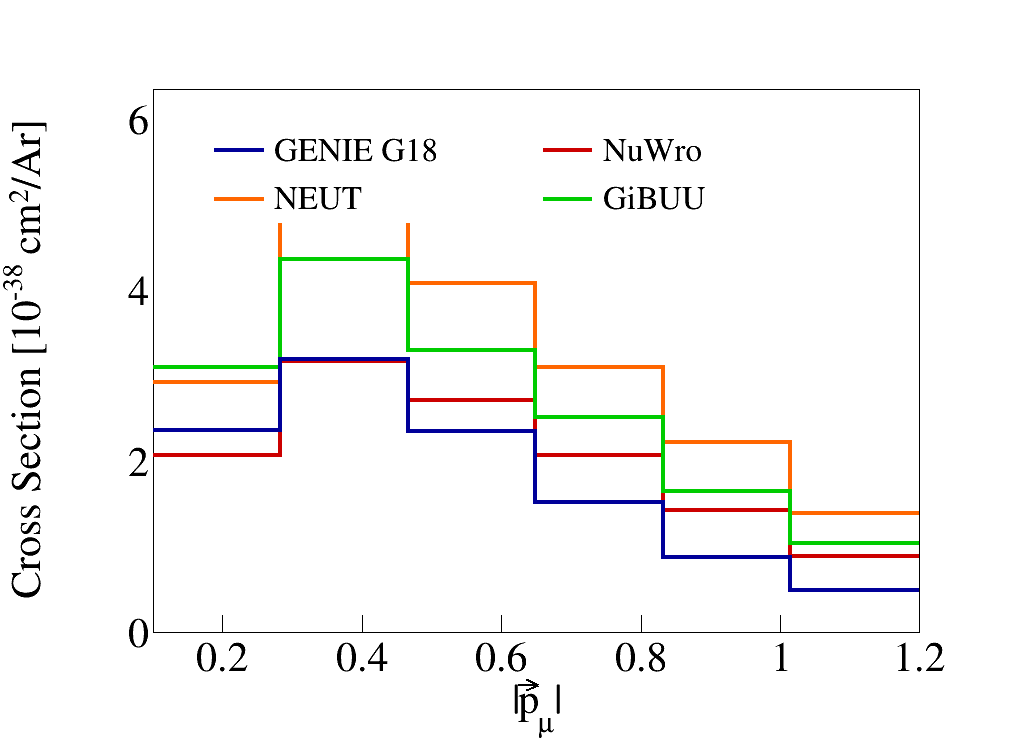
\includegraphics[width=3in]{Figs/Overlay/PostFSI/Overlay_TrueMuonMomentumPlot.png}}
    \subfloat{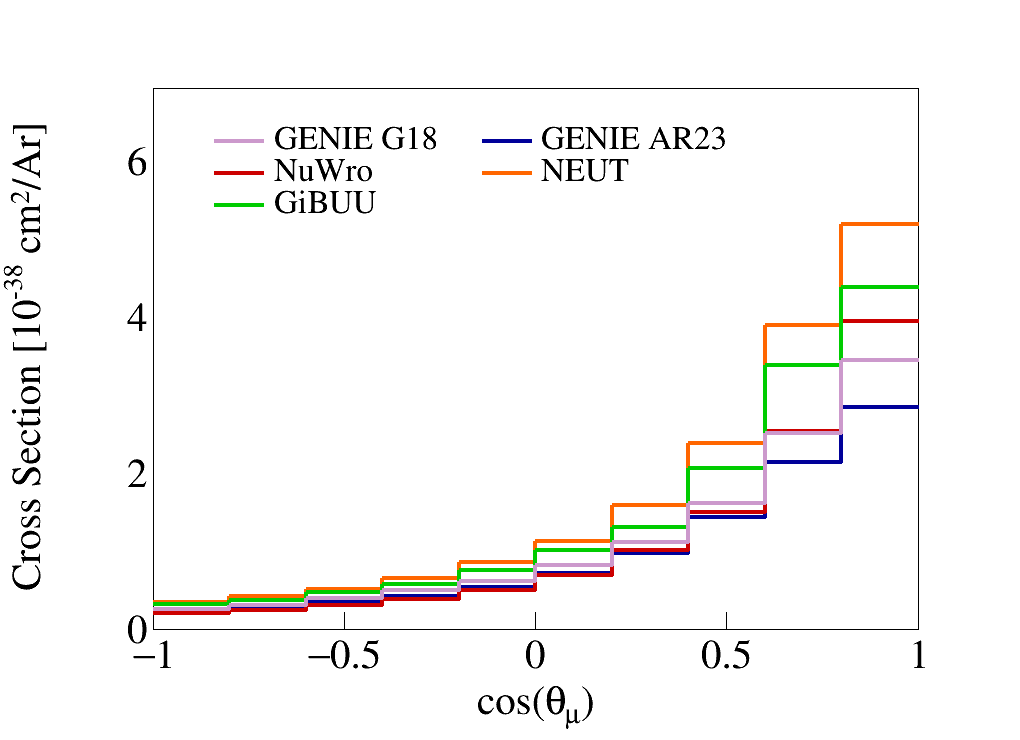
\includegraphics[width=3in]{Figs/Overlay/PostFSI/Overlay_TrueMuonCosThetaPlot.png}} \\
    \subfloat{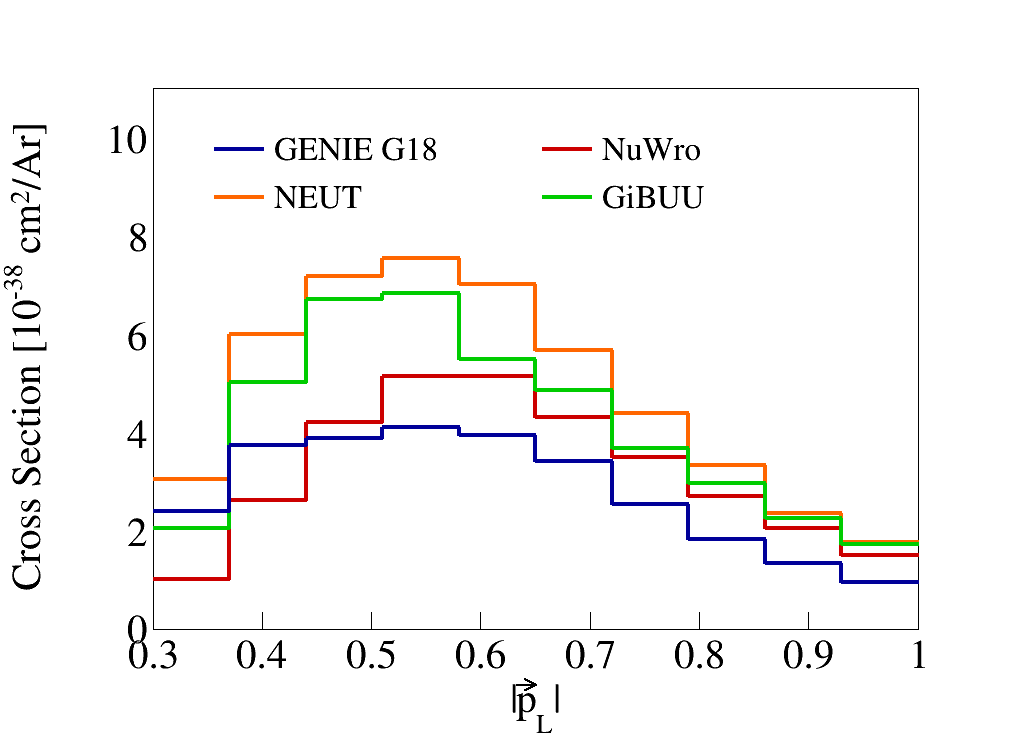
\includegraphics[width=3in]{Figs/Overlay/PostFSI/Overlay_TrueLeadingProtonMomentumPlot.png}}
    \subfloat{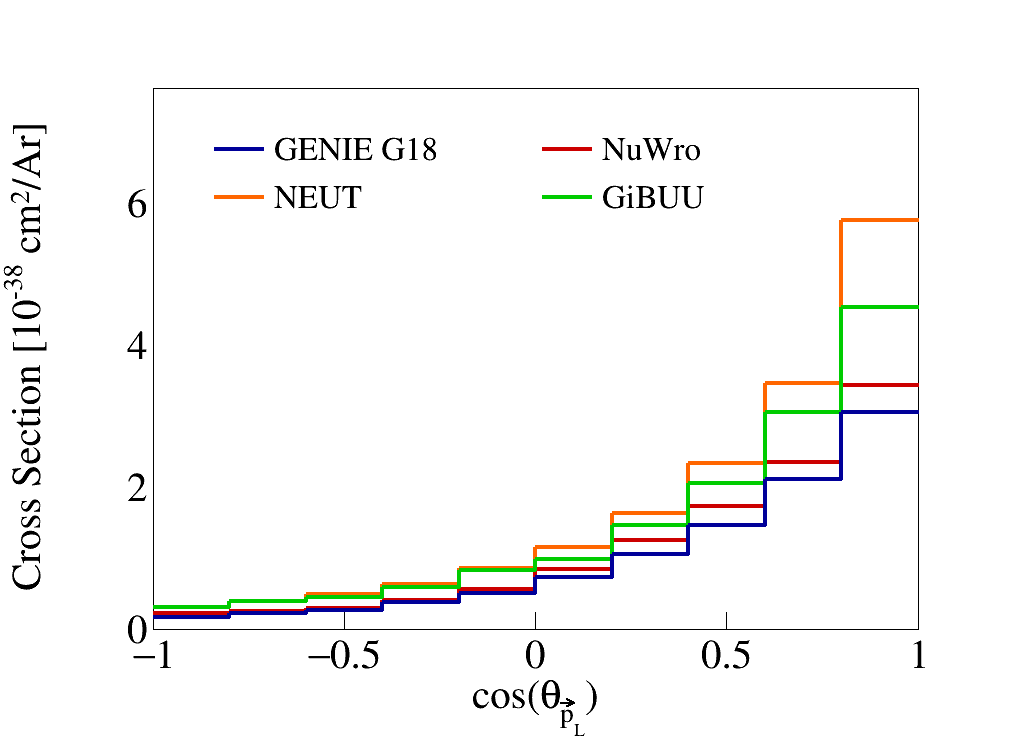
\includegraphics[width=3in]{Figs/Overlay/PostFSI/Overlay_TrueLeadingProtonCosThetaPlot.png}} \\
    \subfloat{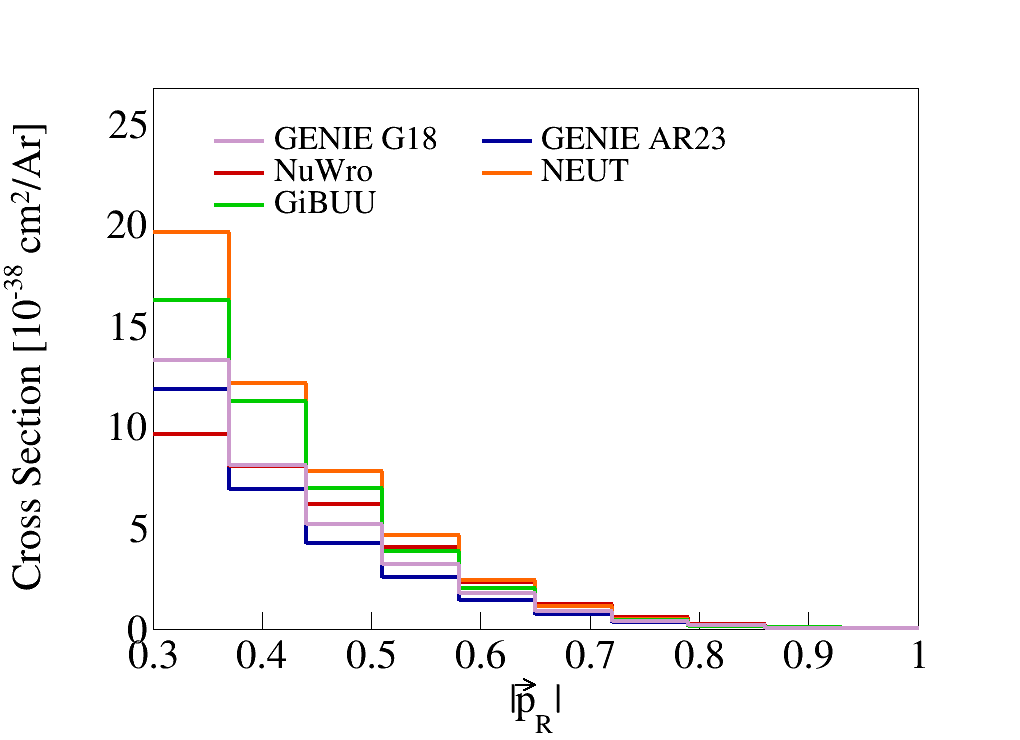
\includegraphics[width=3in]{Figs/Overlay/PostFSI/Overlay_TrueRecoilProtonMomentumPlot.png}}
    \subfloat{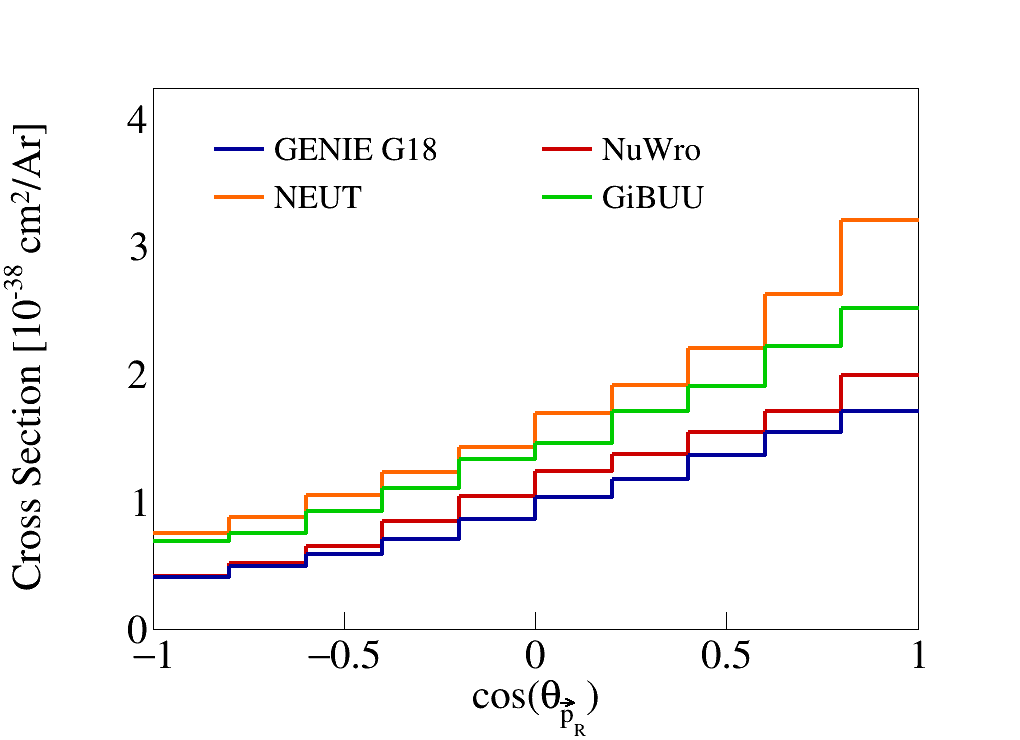
\includegraphics[width=3in]{Figs/Overlay/PostFSI/Overlay_TrueRecoilProtonCosThetaPlot.png}} \\
    \caption{Cross sections for momenta and angles of individual particles}
    \label{fig:momenta-cos-theta}
\end{figure}

We also define variables relating the multiple momentum vectors. First, the opening angle between the protons in the lab frame,
given by 
\begin{align}
    \cos\left(\theta_{\vlp,\vrp}\right) = \frac{\vlp \cdot \vrp}{|\vlp||\vrp|}.
\end{align}
Then, the opening angle between the total proton momentum ($\vtp = \vlp + \vrp$) and the 
muon, given by 
\begin{align}
    \cos\left(\theta_{\vm,\vtp}\right) = \frac{\vm \cdot \vtp}{|\vm||\vtp|}.
\end{align}
Finally, the momentum transverse to the direction of the neutrino beam, which we denote $\vdp$ and is given by 
\begin{align}
    \vdp = \vec{p}^{\mu}_T + \vec{p}^{L}_T + \vec{p}^{R}_T.
\end{align}
For the transverse momentum, we will be interested in its magnitude $|\vdp|$. We plot the differential cross sections of these variables against for the given generators in Figure~\ref{fig:angles-transverse-momentum}. We can also see the cross section by event type for $|\vdp|$ for the NuWro and GENIE AR23 generators in Figure~\ref{fig:inte-breakdown-dpt}.

\begin{figure}
    \centering
    \subfloat{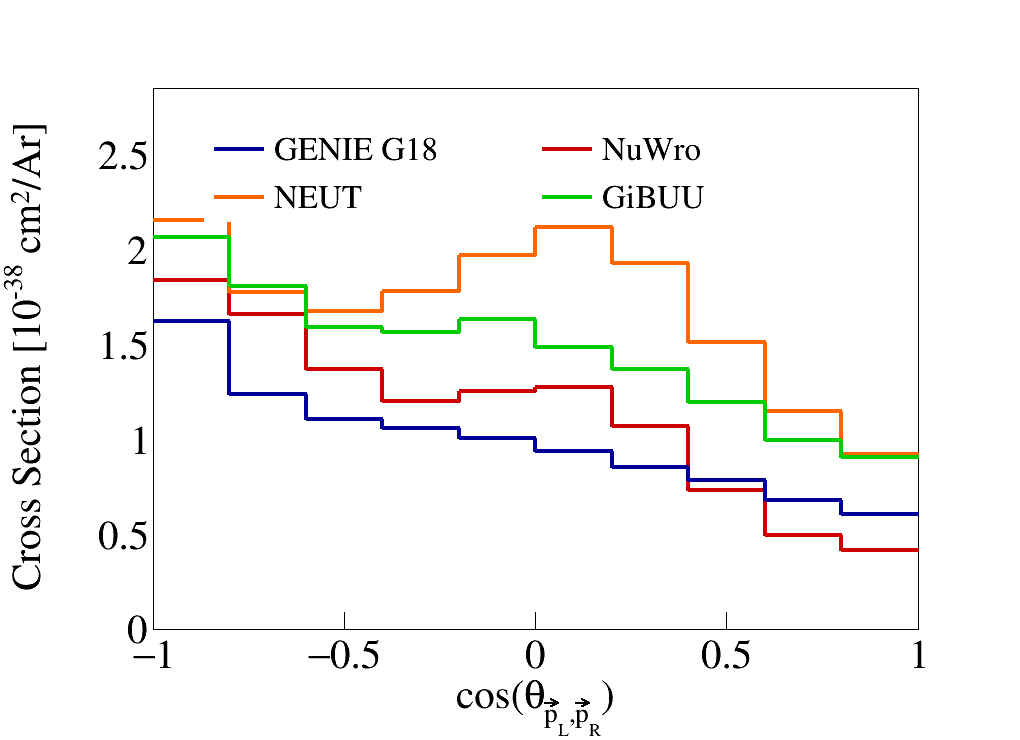
\includegraphics[width=3in]{Figs/Overlay/PostFSI/Overlay_TrueCosOpeningAngleProtonsPlot.png}}
    \subfloat{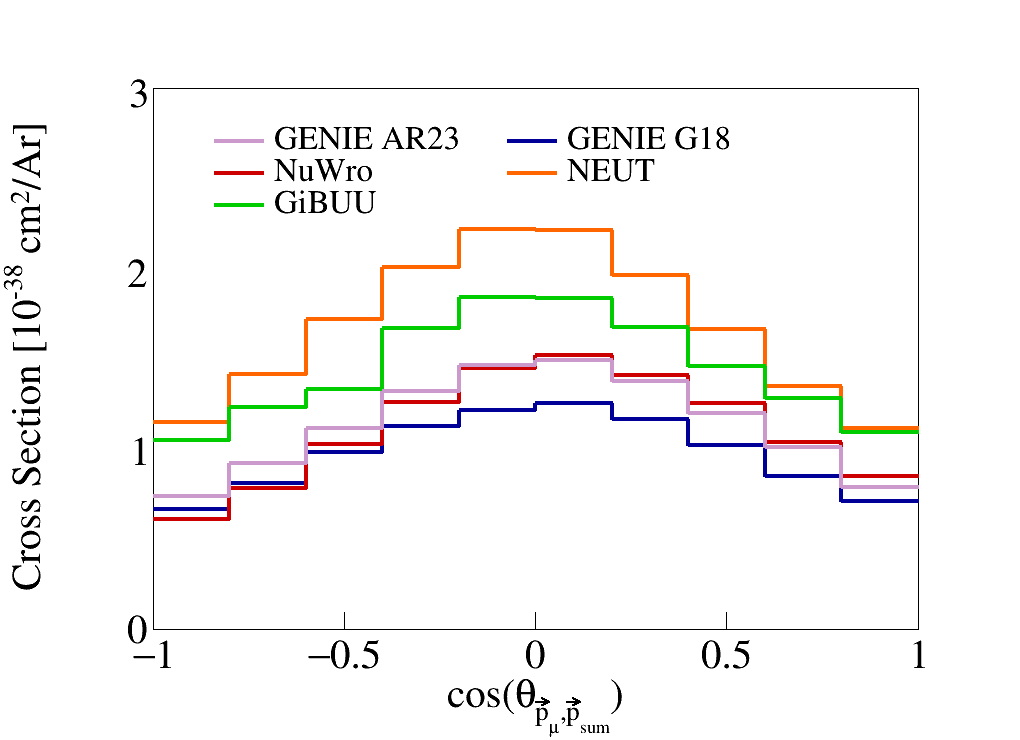
\includegraphics[width=3in]{Figs/Overlay/PostFSI/Overlay_TrueCosOpeningAngleMuonTotalProtonPlot.png}} \\
    \subfloat{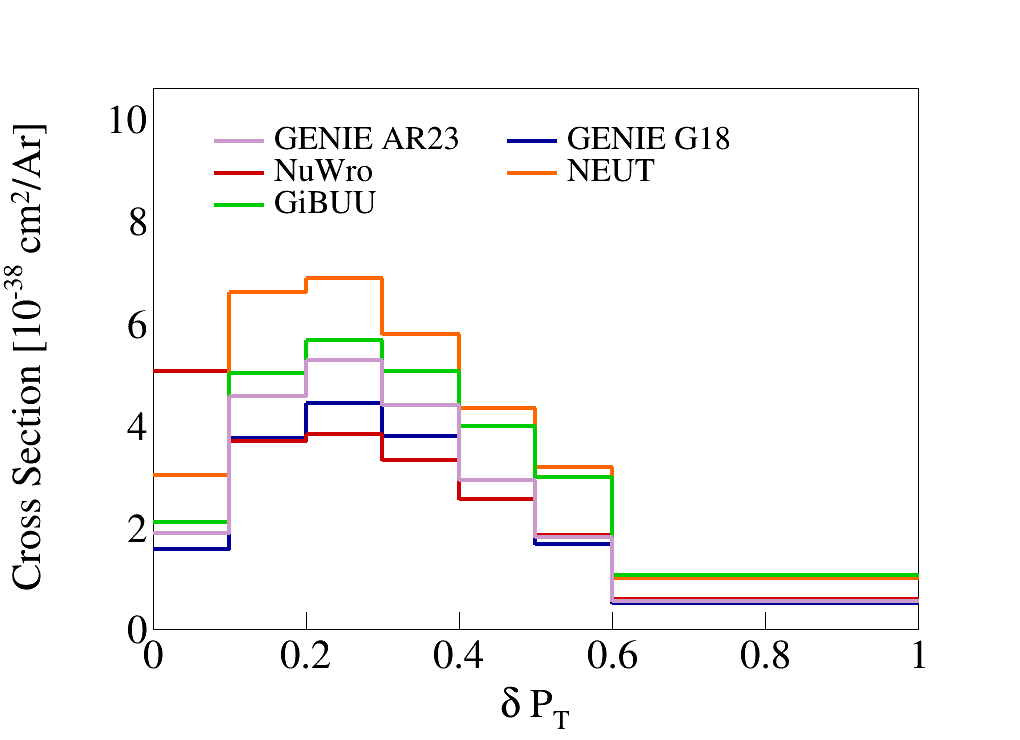
\includegraphics[width=3in]{Figs/Overlay/PostFSI/Overlay_TrueTransverseMomentumPlot.png}}
    \caption{Cross sections for opening angles and transverse momentum.}
    \label{fig:angles-transverse-momentum}
\end{figure}

\begin{figure}
    \centering
    \subfloat{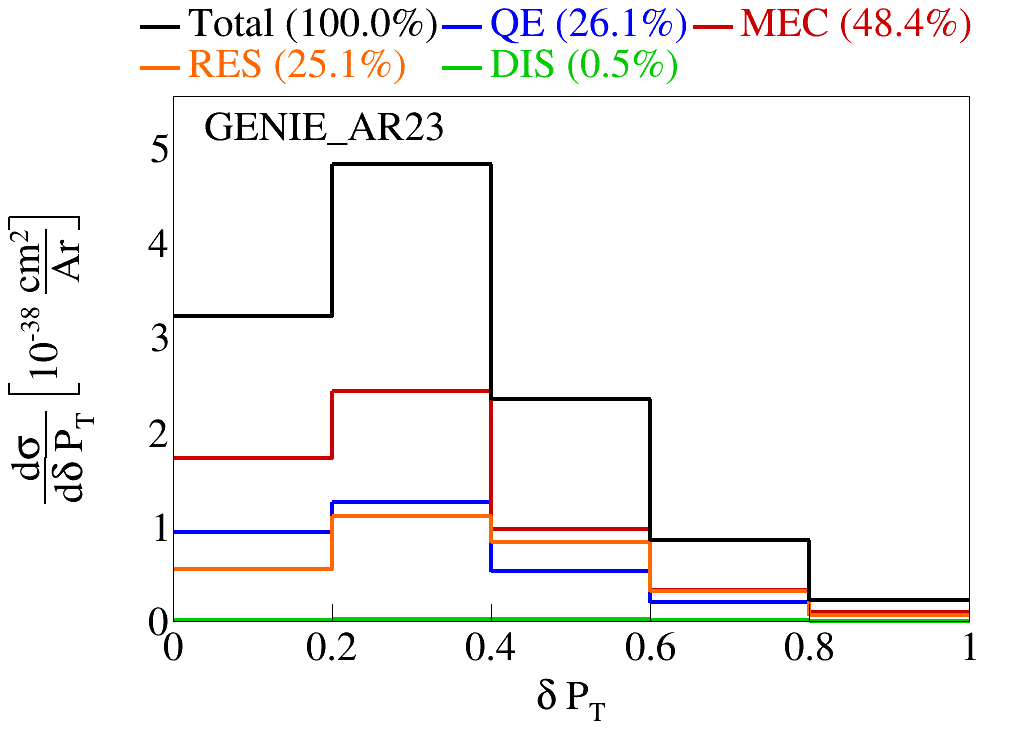
\includegraphics[width=3in]{Figs/InteBreakDown/PostFSI/InteBreakDown_GENIE_AR23_TrueTransverseMomentumPlot.png}}
    \subfloat{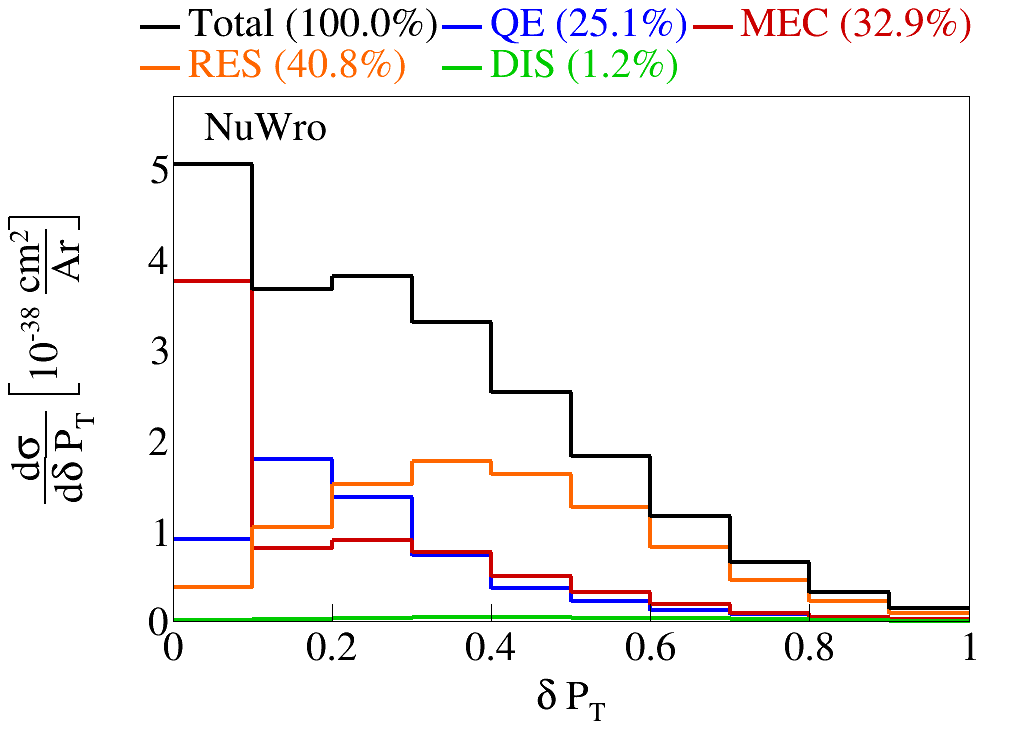
\includegraphics[width=3in]{Figs/InteBreakDown/PostFSI/InteBreakDown_NuWro_TrueTransverseMomentumPlot.png}}
    \caption{Event interaction breakdown for $|\vdp|$.}
    \label{fig:inte-breakdown-dpt}
\end{figure}

\section{Pre-FSI events}

To investigate why the percentage of MEC events for some generators is low, we performed event selection before any final state interactions took place. For both GENIE tunes, NEUT, and NuWro, we got 100\% MEC events pre-FSI. For GiBUU, only 4.1\% MEC versus 76.2\% RES and 16\% DIS events pre-FSI. The plots for GiBUU and NuWro are shown in Figure~\ref{fig:pre-fsi-inte-breakdown}. 

Since GiBUU is the outlier, we checked the specific interaction mode for the RES events. We got that 10 has 39.3\%, 11 has 34.7\%, 12 has 0.0136\%, 13 has 26 \%, and 27, 22, and 23 all have zero percent of the RES events. We also checked the event interaction breakdown for GiBUU samples without final state interactions, in which we found that 100\% of the events are MEC, shown in Figure~\ref{fig:gibuu-no-fsi}.

\begin{figure}
    \centering
    \subfloat{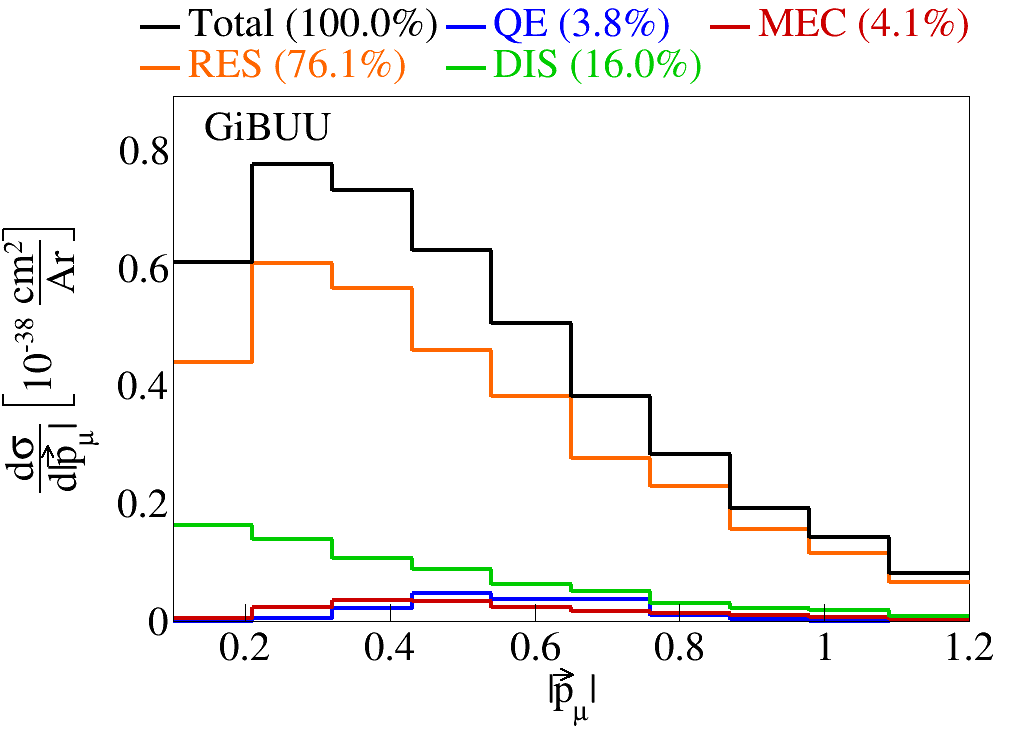
\includegraphics[width=3in]{Figs/InteBreakDown/PreFSI/InteBreakDown_GiBUU_TrueNoFSIMuonMomentumPlot.png}}
    \subfloat{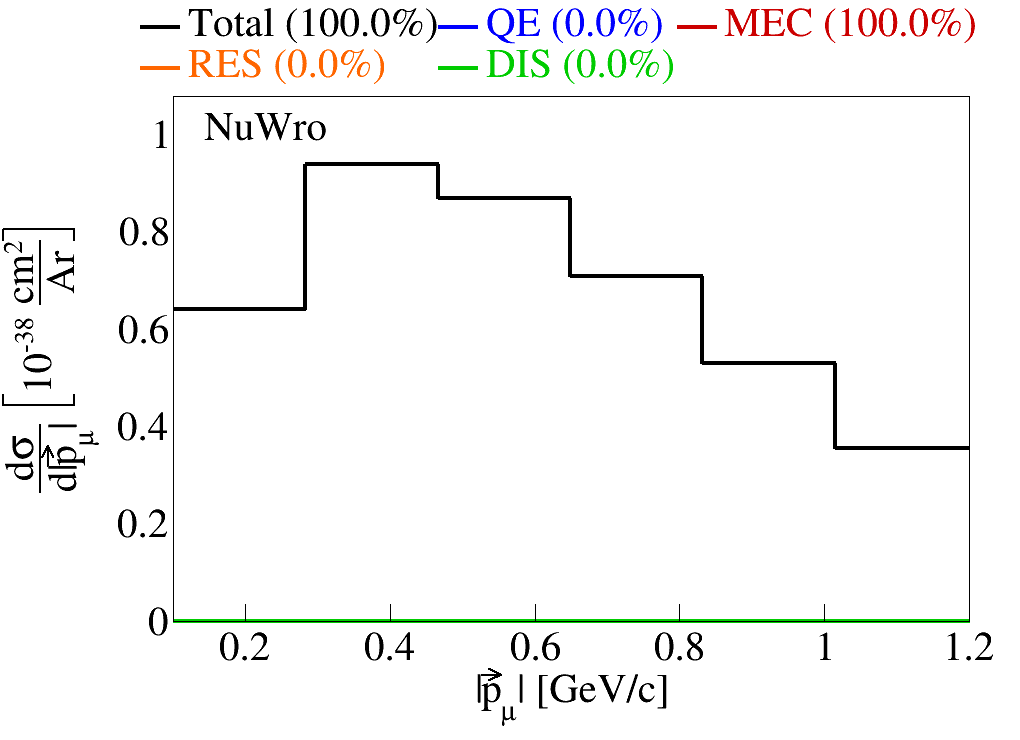
\includegraphics[width=3in]{Figs/InteBreakDown/PreFSI/InteBreakDown_NuWro_TrueNoFSIMuonMomentumPlot.png}}
    \caption{Event interaction breakdown before final state interactions}
    \label{fig:pre-fsi-inte-breakdown}
\end{figure}

\begin{figure}
    \centering
    \subfloat{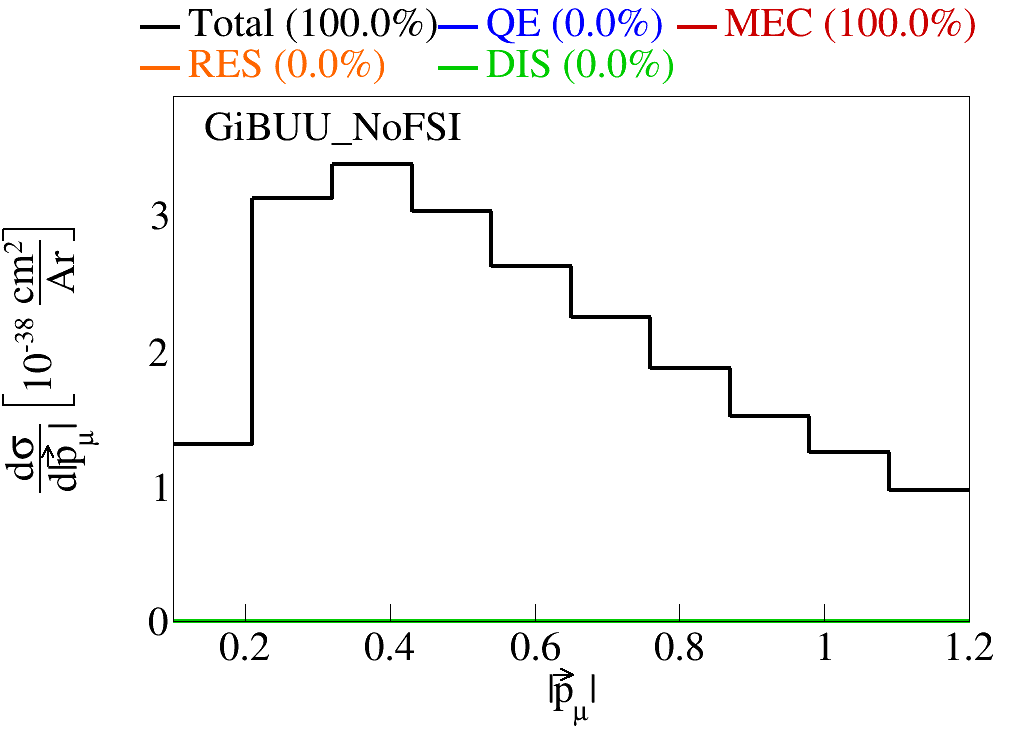
\includegraphics[width=3in]{Figs/InteBreakDown/PostFSI/InteBreakDown_GiBUU_NoFSI_TrueMuonMomentumPlot.png}}
    \caption{Event interaction breakdown for final events from GiBUU events with no FSI}
    \label{fig:gibuu-no-fsi}
\end{figure}

\section{Double differential plots}

We plot $\delta P_T$, $\delta \alpha_T$, $\cos\left(\theta_{\vlp,\vrp}\right)$, and $\cos\left(\theta_{\vm,\vtp}\right)$ in $\cos(\theta_{\vec{p}_{\mu}})$. These are shown in Figure~\ref{fig:double-differential-cos-mu}. We have two bins for $\cos(\theta_{\vec{p}_{\mu}})$, the first one going from $-1$ to $0.5$ and the second from $0.5$ to $1$. Therefore, these are irregular bins, with the first holding a larger range than the first.

\begin{figure}
    \centering
    \subfloat{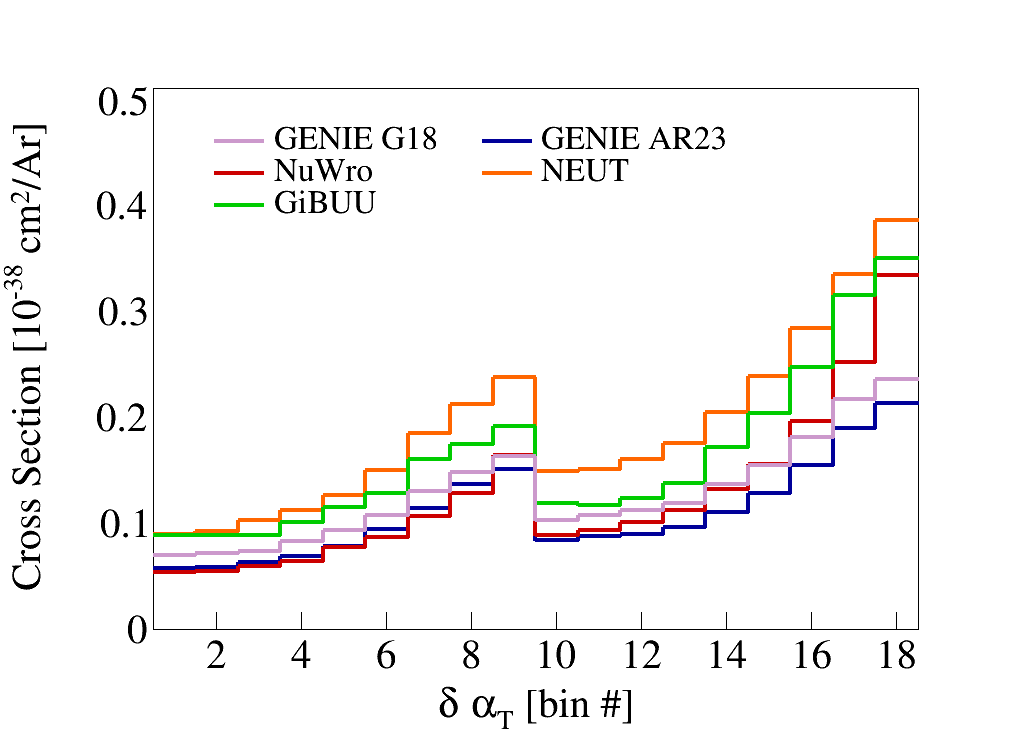
\includegraphics[width=3in]{Figs/Overlay/PostFSI/Overlay_TrueSerialDeltaAlphaT_InMuonCosThetaPlot.png}}
    \subfloat{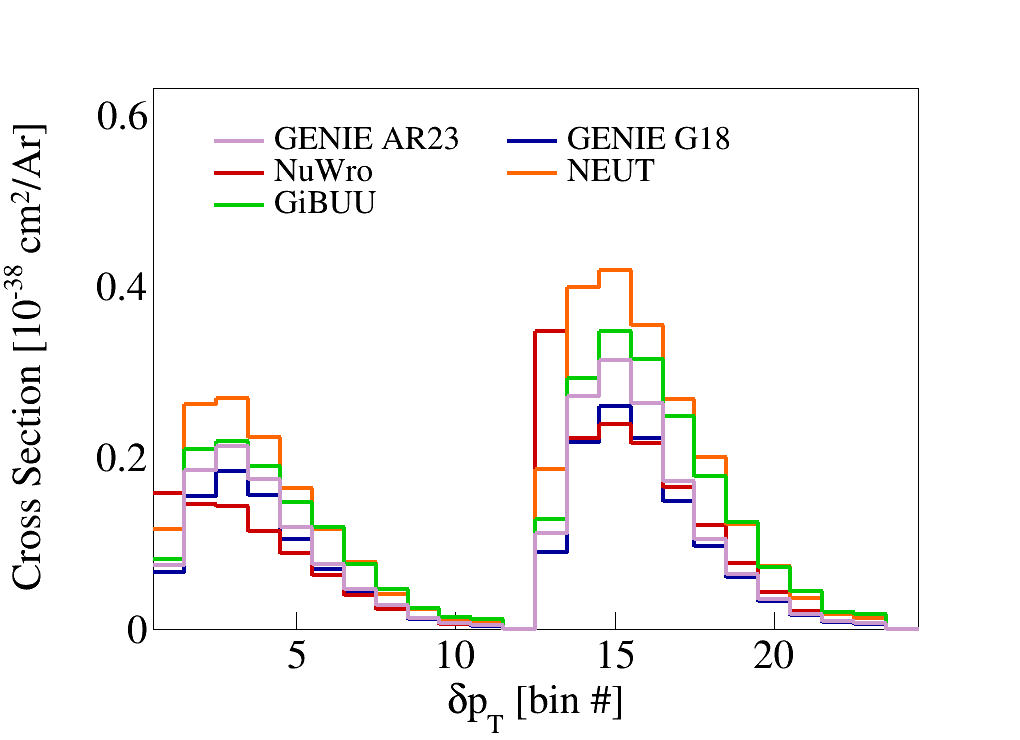
\includegraphics[width=3in]{Figs/Overlay/PostFSI/Overlay_TrueSerialTransverseMomentum_InMuonCosThetaPlot.png}} \\
    \subfloat{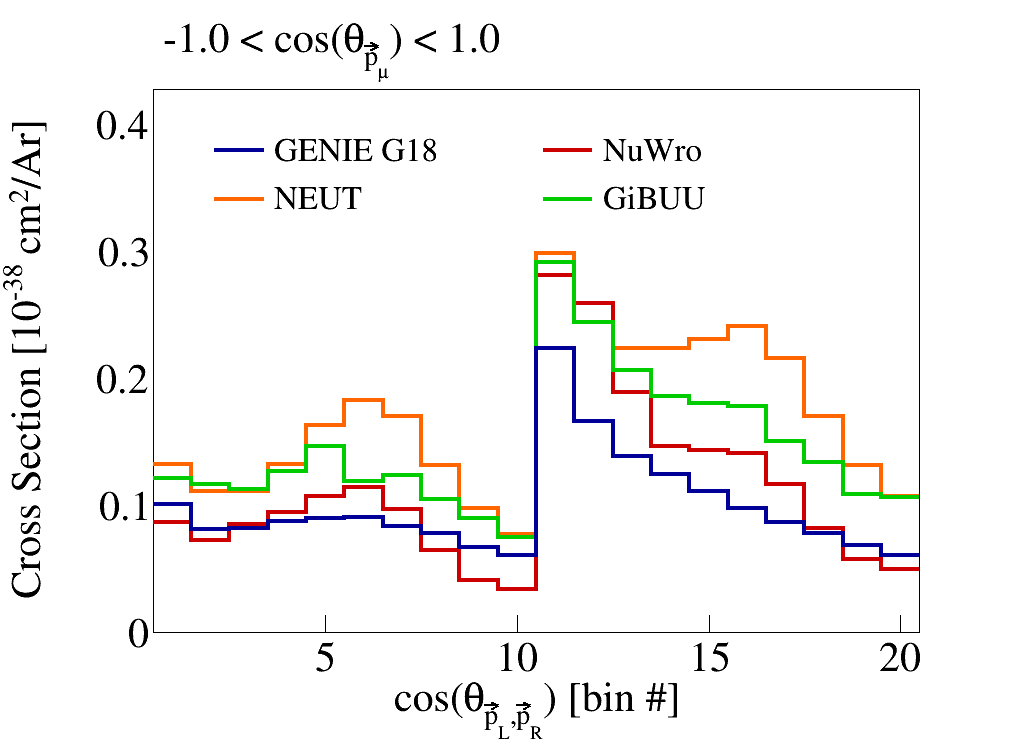
\includegraphics[width=3in]{Figs/Overlay/PostFSI/Overlay_TrueSerialCosOpeningAngleProtons_InMuonCosThetaPlot.png}}
    \subfloat{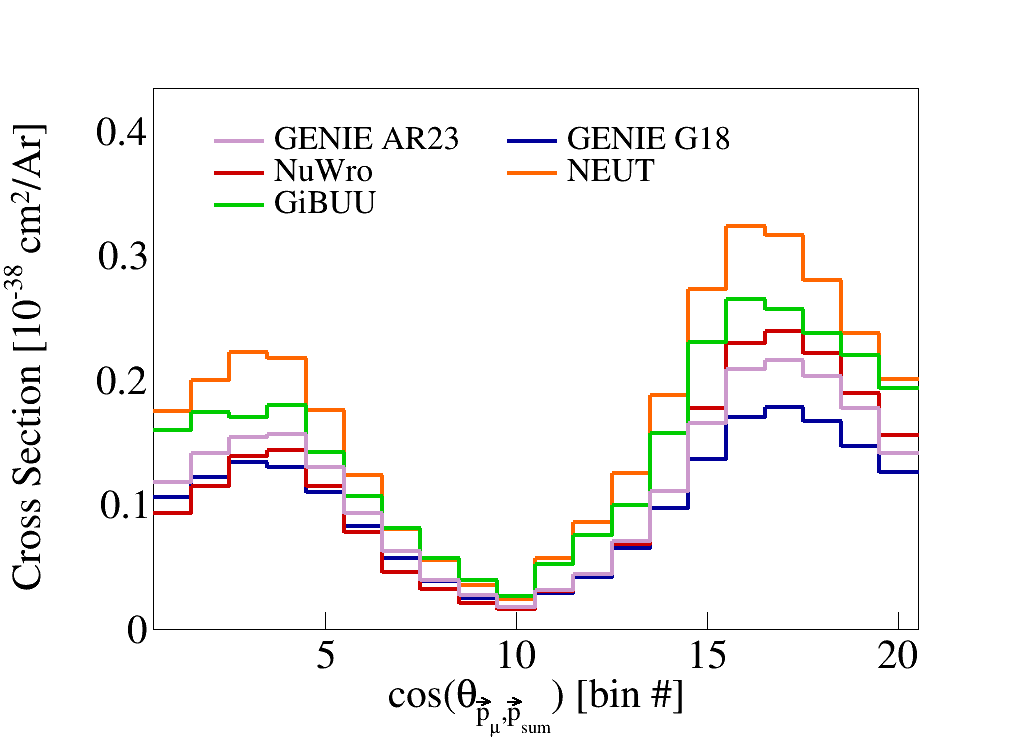
\includegraphics[width=3in]{Figs/Overlay/PostFSI/Overlay_TrueSerialCosOpeningAngleMuonTotalProton_InMuonCosThetaPlot.png}}
    \caption{Double differential plots, all in $\cos(\theta_{\vec{p}_{\mu}})$}
    \label{fig:double-differential-cos-mu}
\end{figure}

We also slice the double differential plots into two plots each, so that we have $\cos(\theta_{\vec{p}_{\mu}})$ in the horizontal axis instead of bin numbers. These plots are shown in Figure~\ref{fig:sliced-double-differential-cos-mu}. In these plots, the bins contents have been reweighed appropriately, by dividing the content of each bin by the width of the bin for the variable in the axis multiplied by the width of the $\cos(\theta_{\vec{p}_{\mu}})$ slice. Note that the plots for the $1 < \cos(\theta_{\vec{p}_{\mu}}) < 1.5$ slice have more events in general, as it can be seen by the scale of the vertical axis. 

\begin{figure}
    \centering
    \subfloat{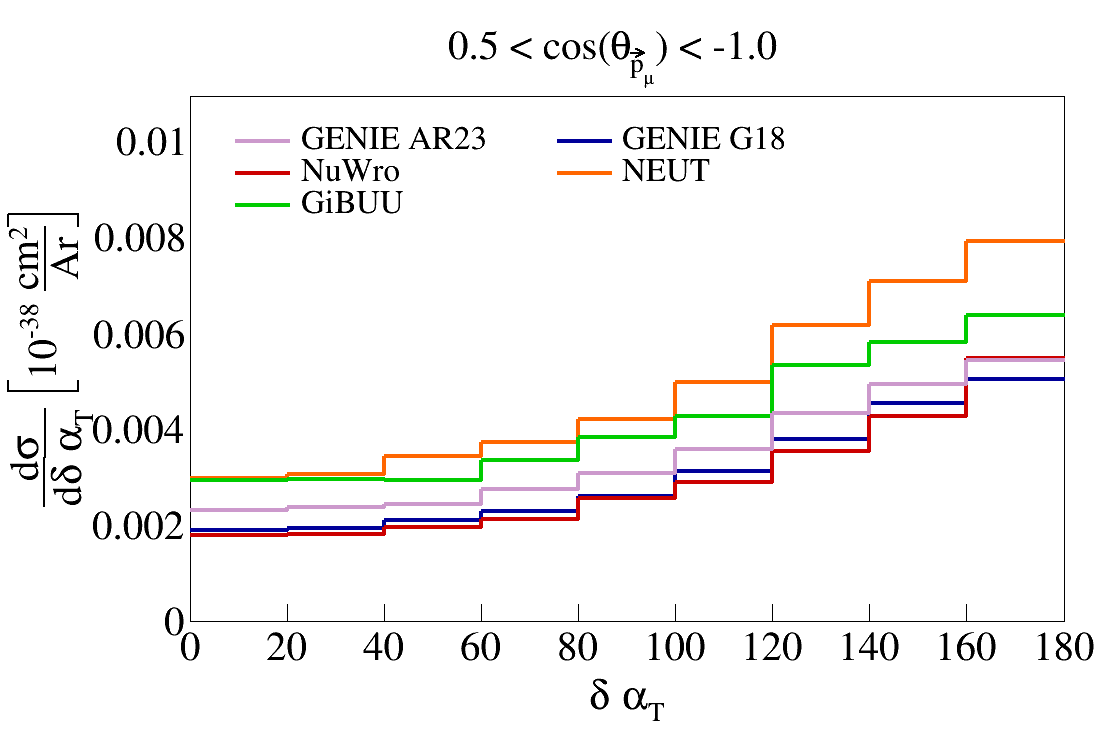
\includegraphics[width=3in]{Figs/Overlay/Serial/TrueSerialDeltaAlphaT_InMuonCosThetaPlot_0.png}}
    \subfloat{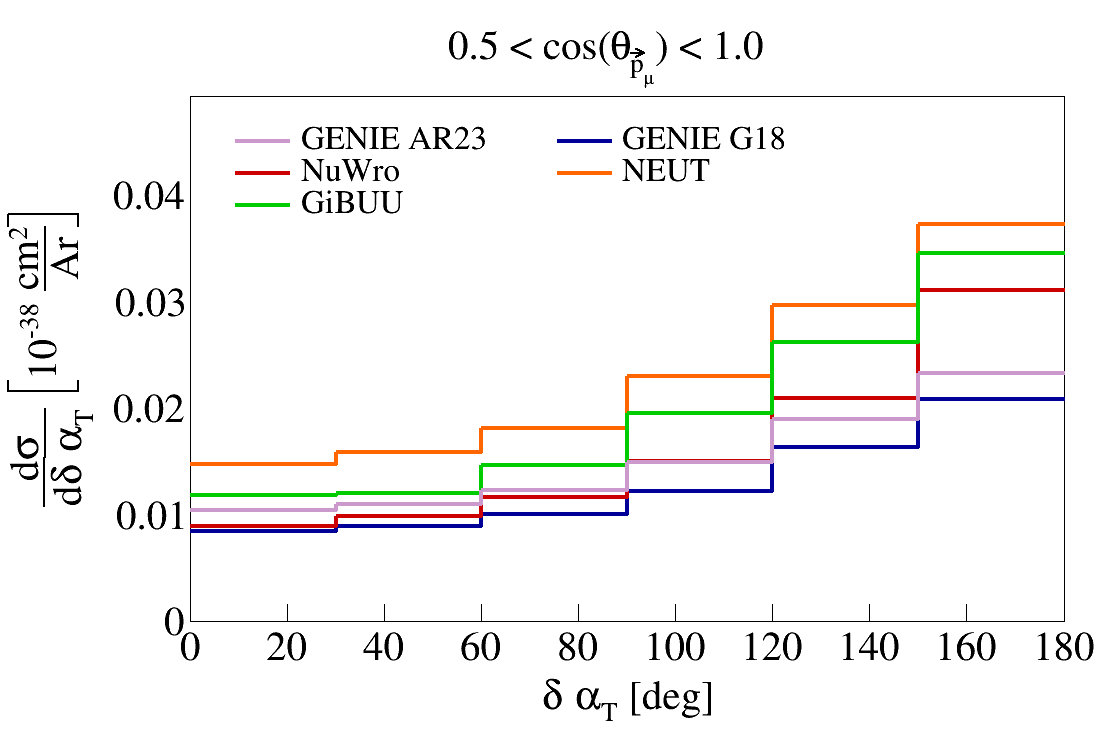
\includegraphics[width=3in]{Figs/Overlay/Serial/TrueSerialDeltaAlphaT_InMuonCosThetaPlot_1.png}} \\
    \subfloat{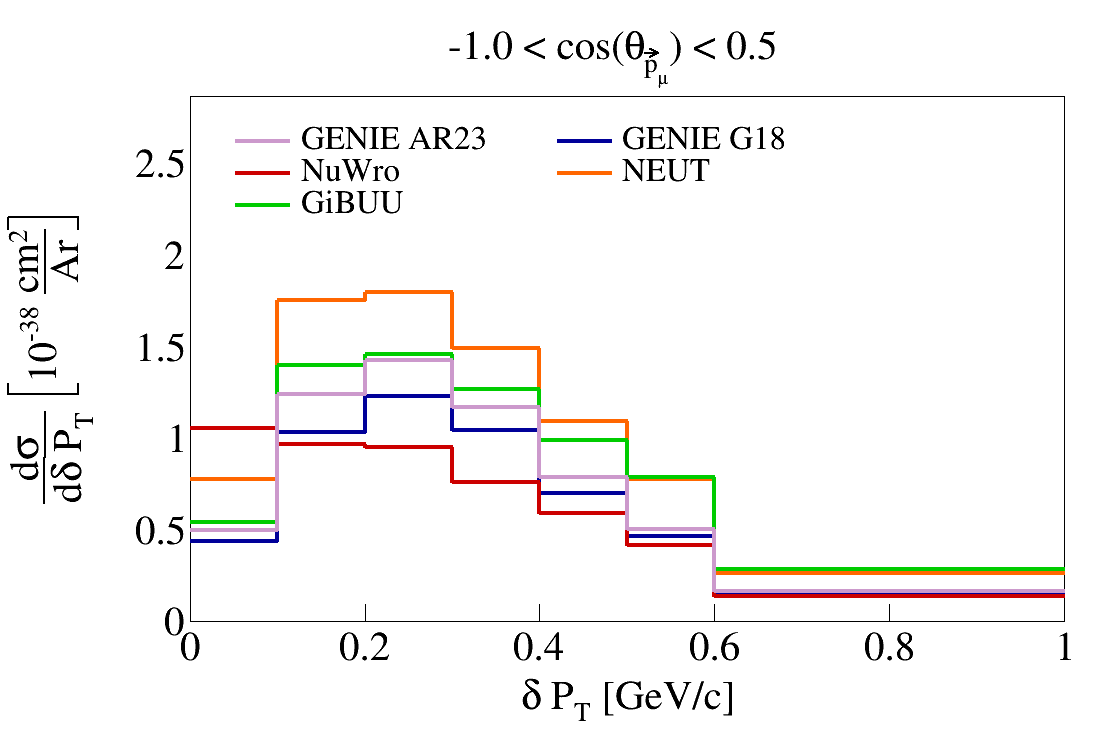
\includegraphics[width=3in]{Figs/Overlay/Serial/TrueSerialTransverseMomentum_InMuonCosThetaPlot_0.png}}
    \subfloat{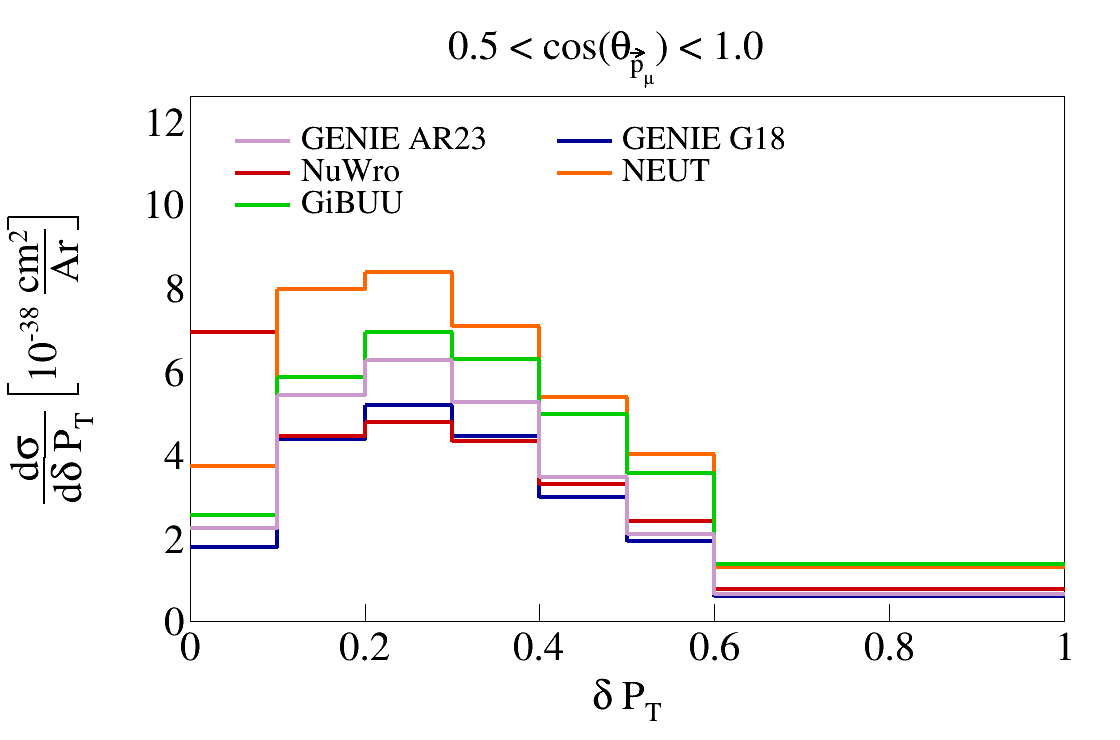
\includegraphics[width=3in]{Figs/Overlay/Serial/TrueSerialTransverseMomentum_InMuonCosThetaPlot_1.png}} \\
    \subfloat{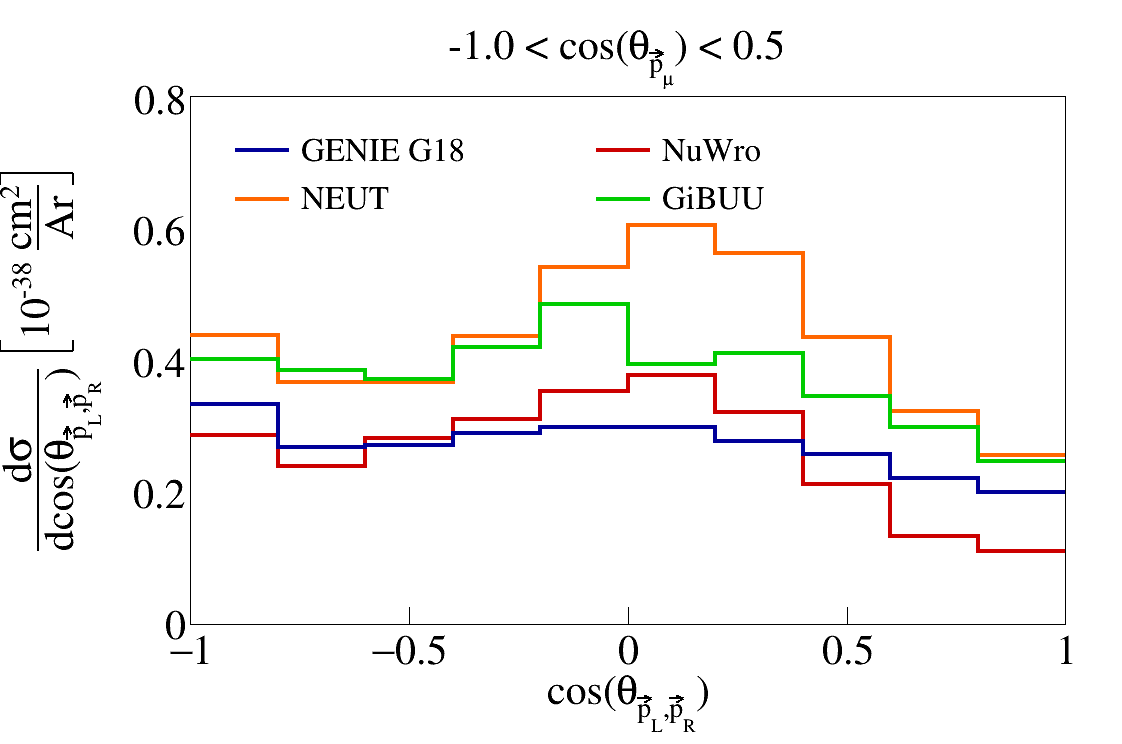
\includegraphics[width=3in]{Figs/Overlay/Serial/TrueSerialCosOpeningAngleProtons_InMuonCosThetaPlot_0.png}}
    \subfloat{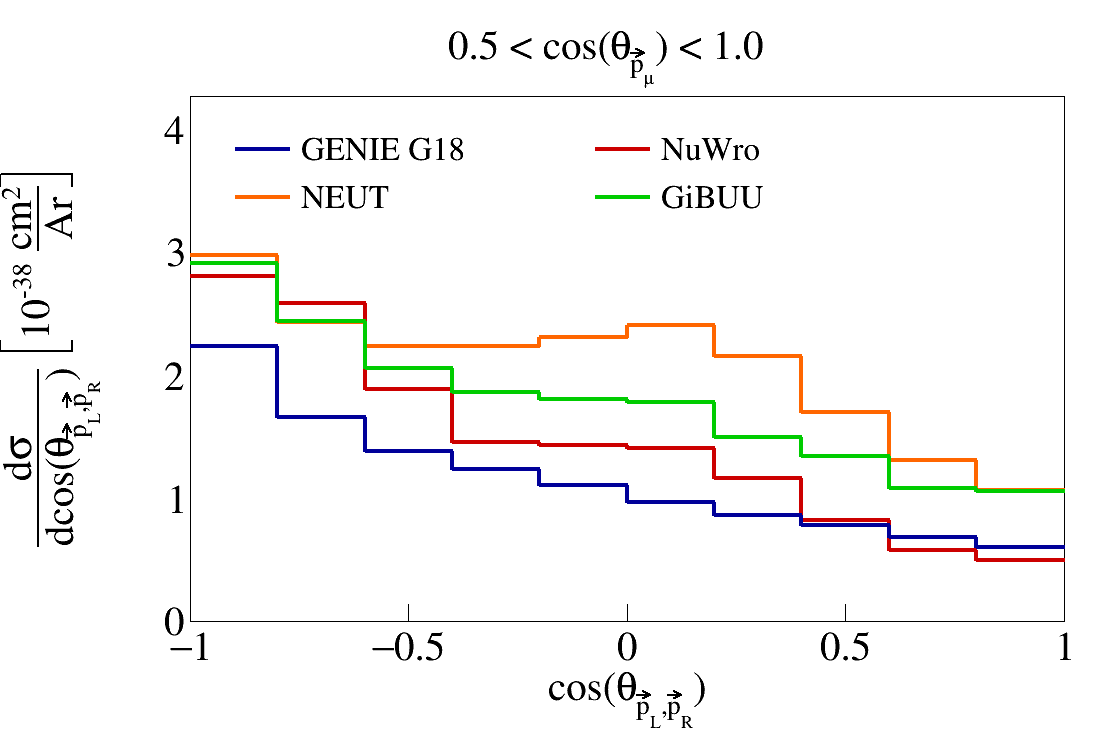
\includegraphics[width=3in]{Figs/Overlay/Serial/TrueSerialCosOpeningAngleProtons_InMuonCosThetaPlot_1.png}} \\
    \subfloat{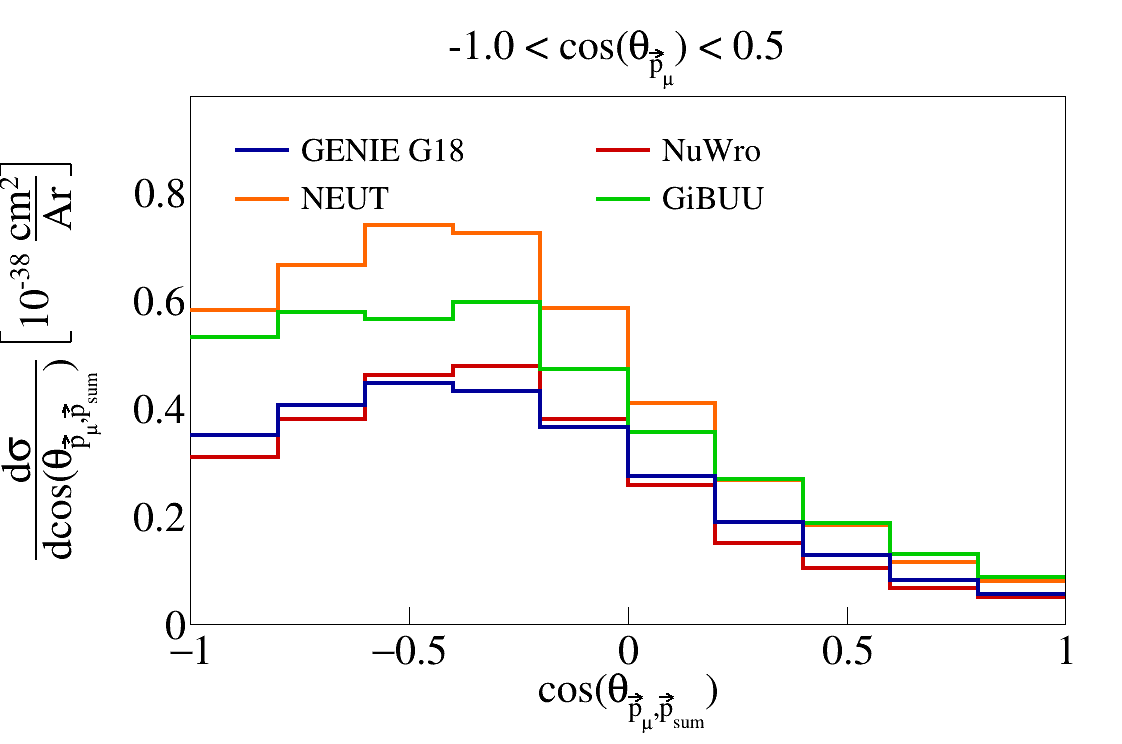
\includegraphics[width=3in]{Figs/Overlay/Serial/TrueSerialCosOpeningAngleMuonTotalProton_InMuonCosThetaPlot_0.png}}
    \subfloat{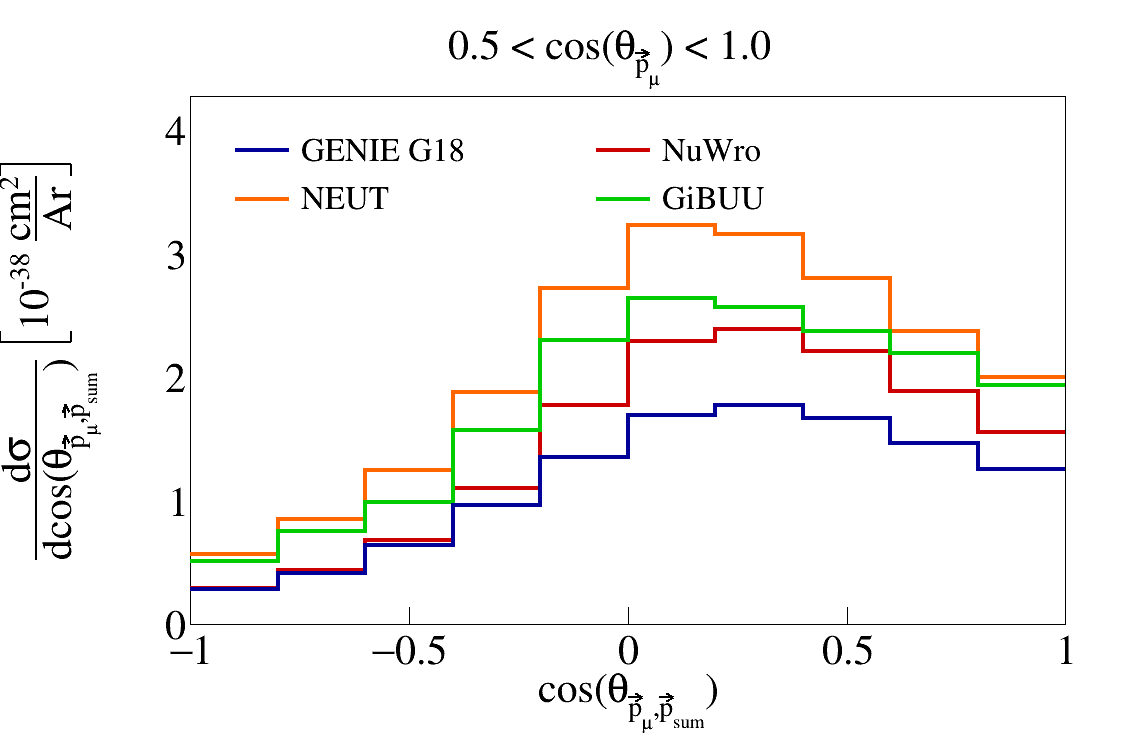
\includegraphics[width=3in]{Figs/Overlay/Serial/TrueSerialCosOpeningAngleMuonTotalProton_InMuonCosThetaPlot_1.png}} 
    \caption{Sliced double differential plots}
    \label{fig:sliced-double-differential-cos-mu}
\end{figure}

We also performed the same double differential analysis but for the events before final state interactions. These are shown in Figure~\ref{fig:sliced-double-differential-cos-mu-no-fsi}. Only the plots for the two opening angles are shown here for compactness. 

\begin{figure}
    \centering
    % \subfloat{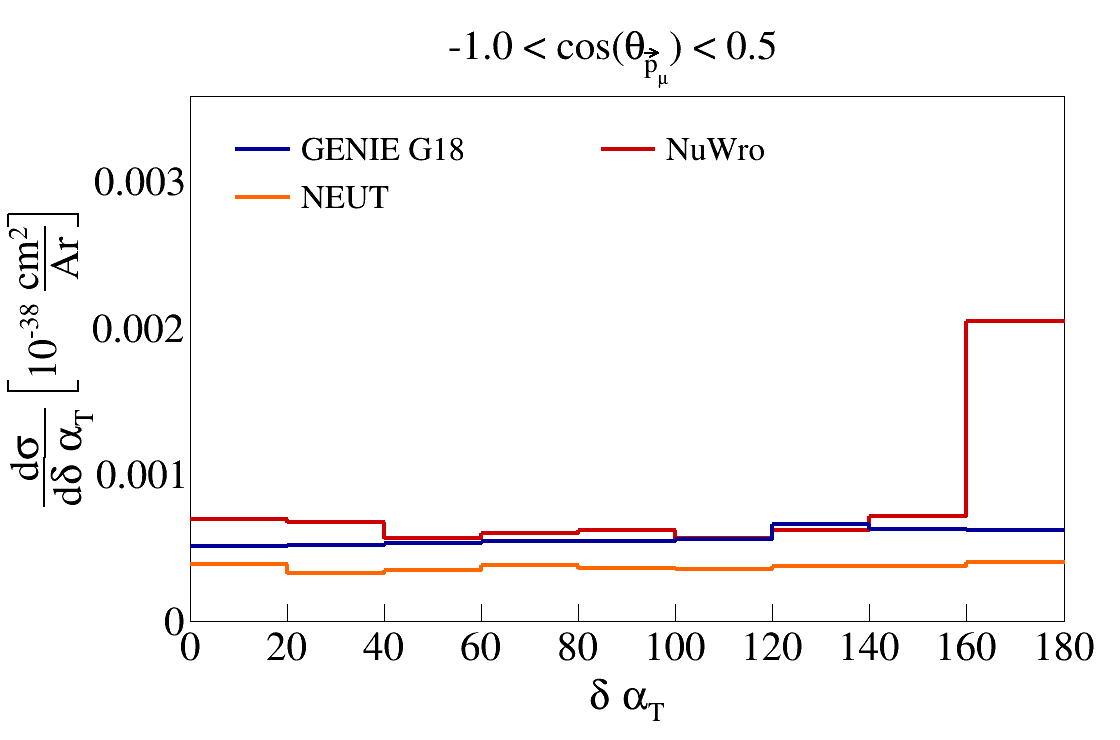
\includegraphics[width=3in]{Figs/Overlay/Serial/TrueSerialNoFSIDeltaAlphaT_InMuonCosThetaPlot_0.png}}
    % \subfloat{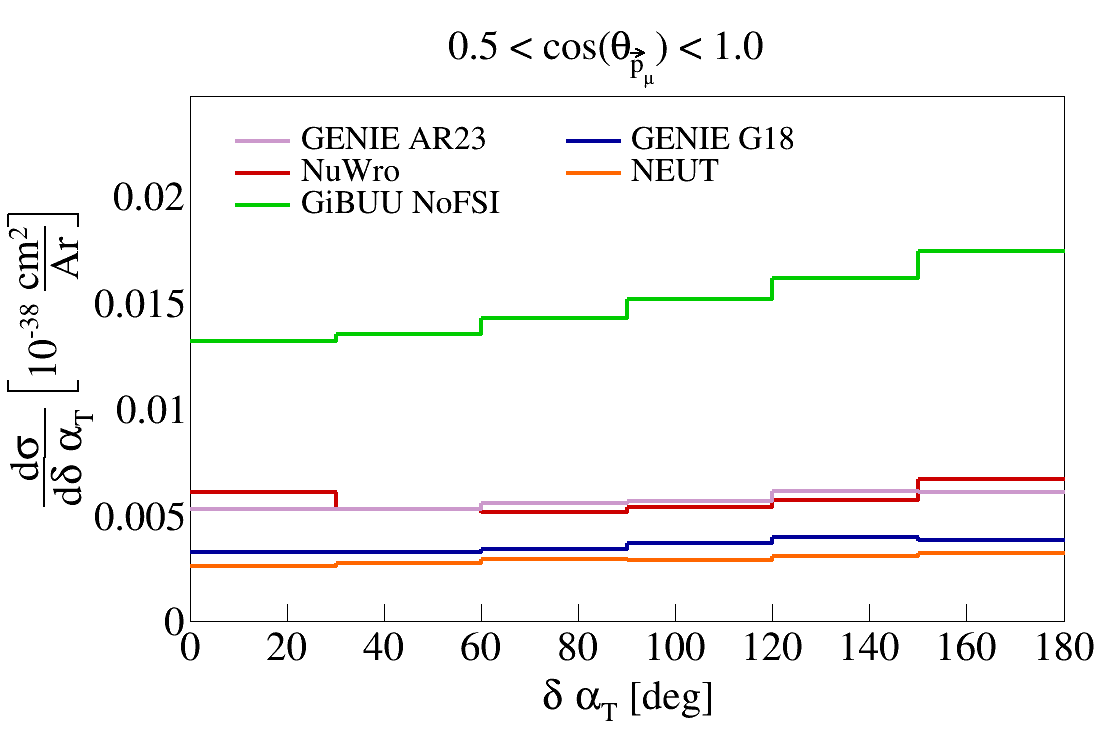
\includegraphics[width=3in]{Figs/Overlay/Serial/TrueSerialNoFSIDeltaAlphaT_InMuonCosThetaPlot_1.png}} \\
    % \subfloat{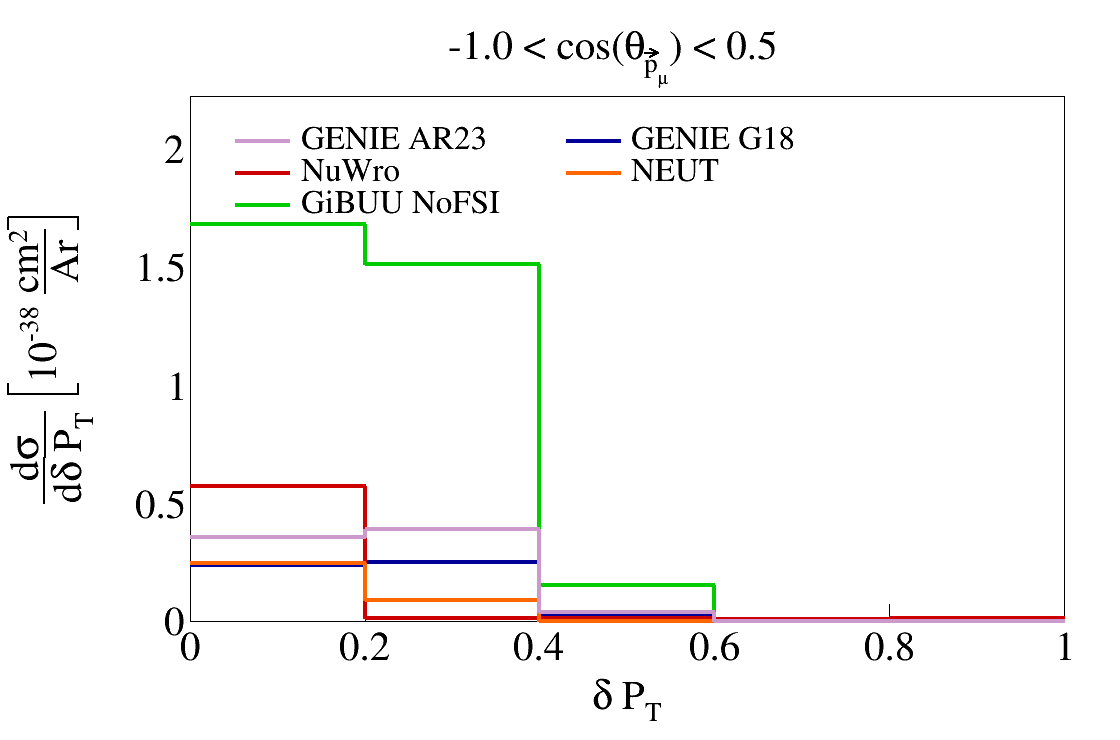
\includegraphics[width=3in]{Figs/Overlay/Serial/TrueSerialNoFSITransverseMomentum_InMuonCosThetaPlot_0.png}}
    % \subfloat{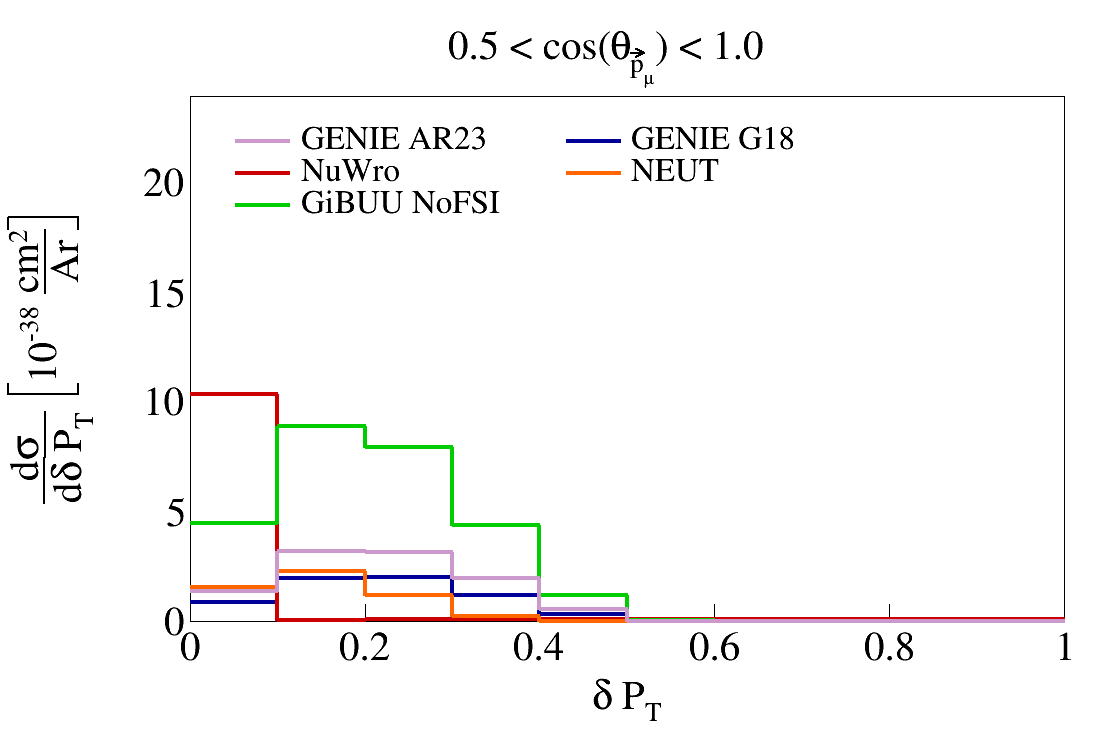
\includegraphics[width=3in]{Figs/Overlay/Serial/TrueSerialNoFSITransverseMomentum_InMuonCosThetaPlot_1.png}} \\
    \subfloat{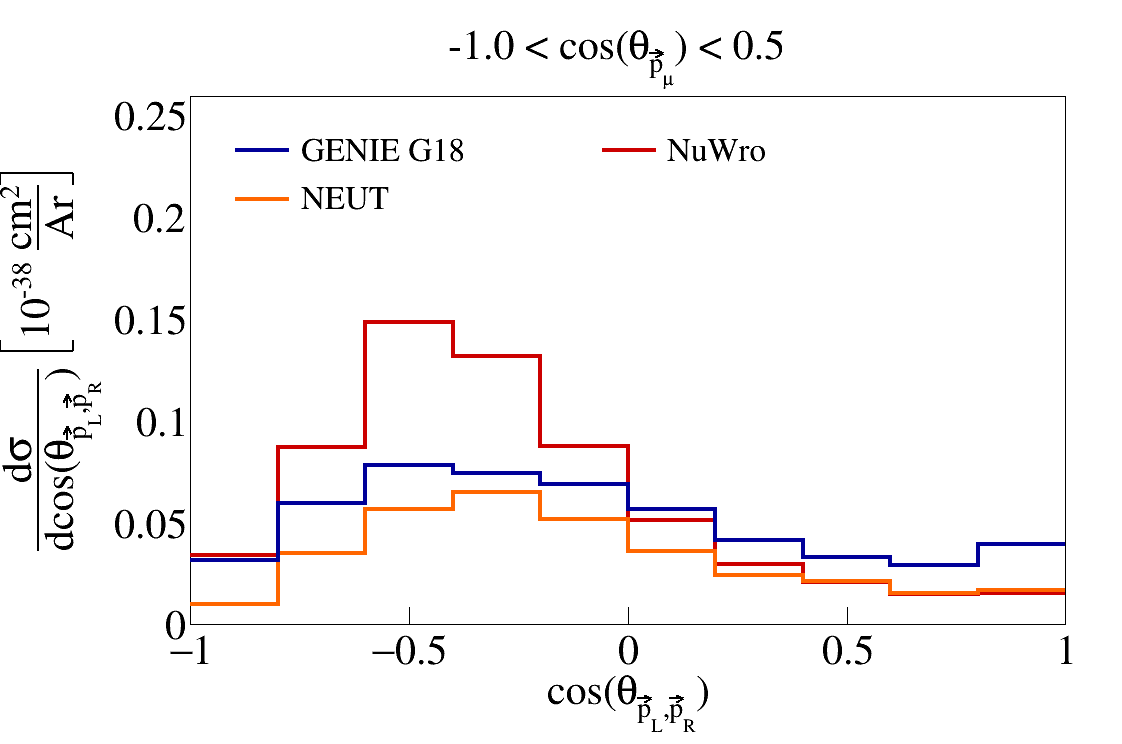
\includegraphics[width=3in]{Figs/Overlay/Serial/TrueSerialNoFSICosOpeningAngleProtons_InMuonCosThetaPlot_0.png}}
    \subfloat{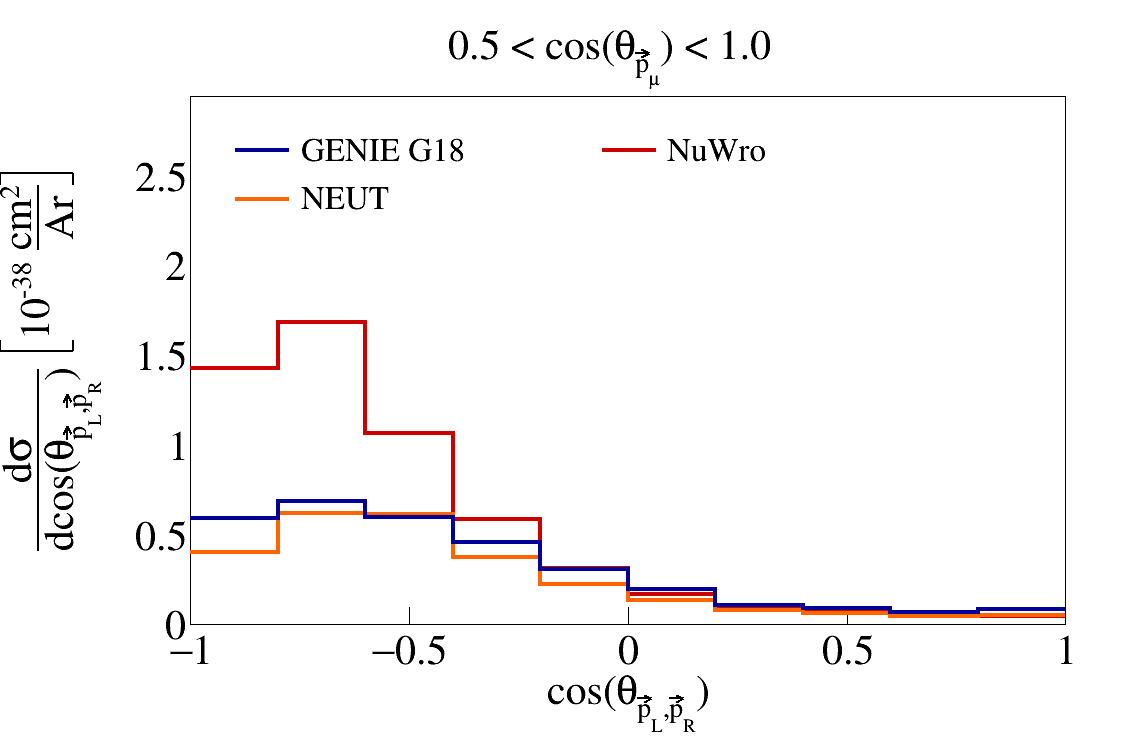
\includegraphics[width=3in]{Figs/Overlay/Serial/TrueSerialNoFSICosOpeningAngleProtons_InMuonCosThetaPlot_1.png}} \\
    \subfloat{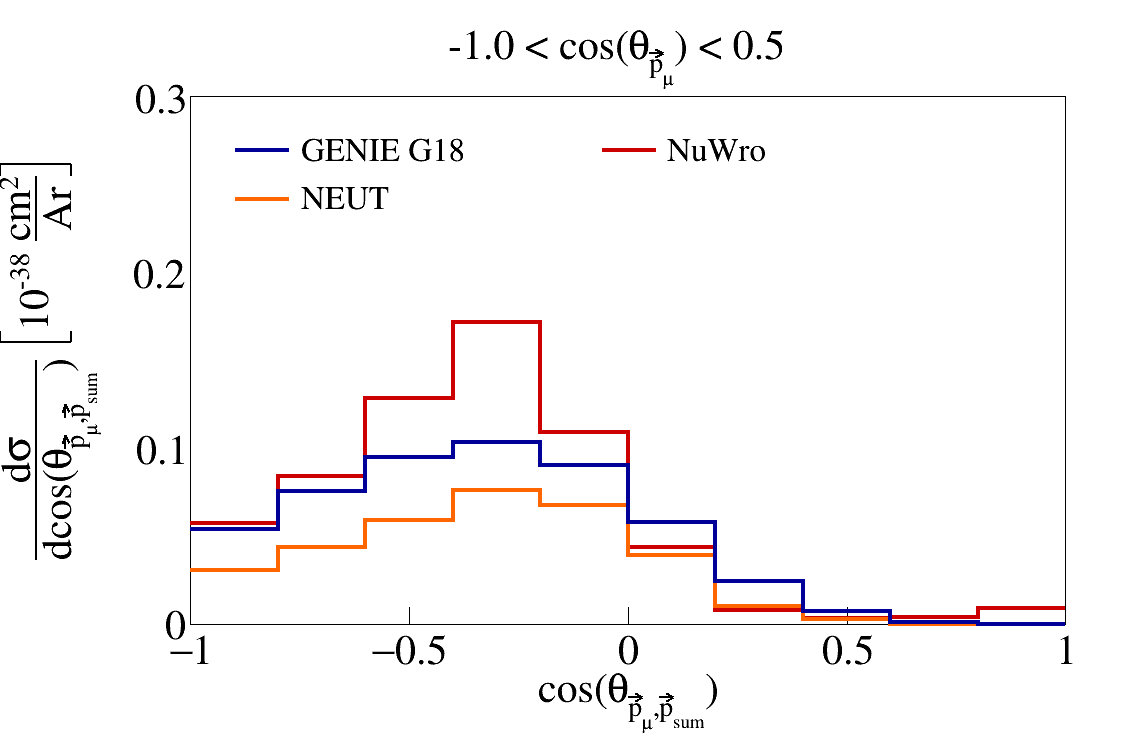
\includegraphics[width=3in]{Figs/Overlay/Serial/TrueSerialNoFSICosOpeningAngleMuonTotalProton_InMuonCosThetaPlot_0.png}}
    \subfloat{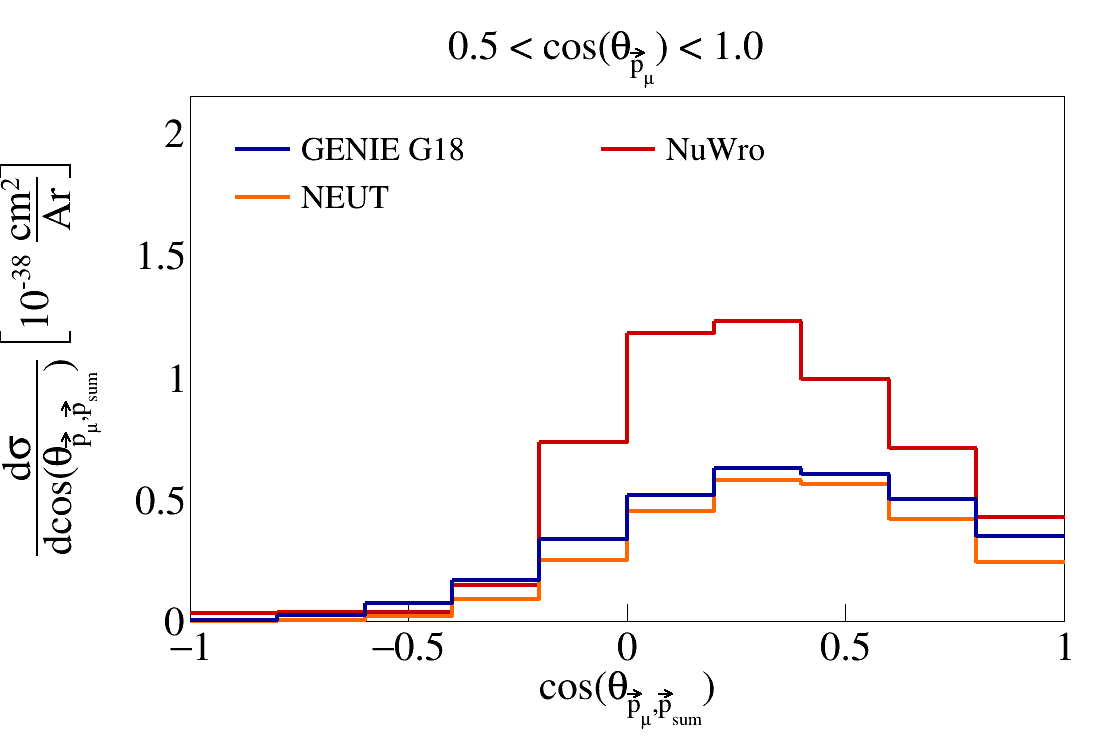
\includegraphics[width=3in]{Figs/Overlay/Serial/TrueSerialNoFSICosOpeningAngleMuonTotalProton_InMuonCosThetaPlot_1.png}} 
    \caption{Sliced double differential plots for pre-FSI events}
    \label{fig:sliced-double-differential-cos-mu-no-fsi}
\end{figure}

\section{Pure MEC events}

We also generated pure MEC events with different configurations to get the MEC splines. These were all different tunes of GENIE: AR23, G18 with Empirical MEC model, and G18 with Nieves MEC model. The plots for the transverse kinematic variables are shown in Figure~\ref{fig:transverse-k-mec}. Some of the sliced double differential plots are shown in Figure~\ref{fig:sliced-double-mec}.

\begin{figure}
    \centering
    \subfloat{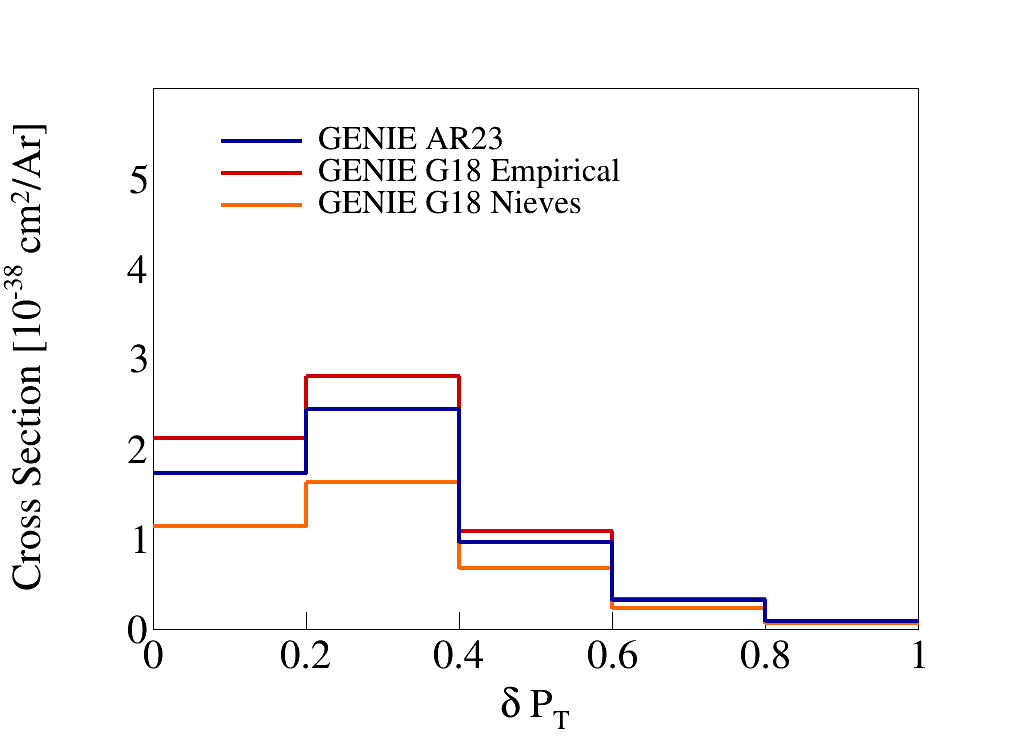
\includegraphics[width=3in]{Figs/Overlay/MEC/Overlay_TrueTransverseMomentumPlot.png}}
    \subfloat{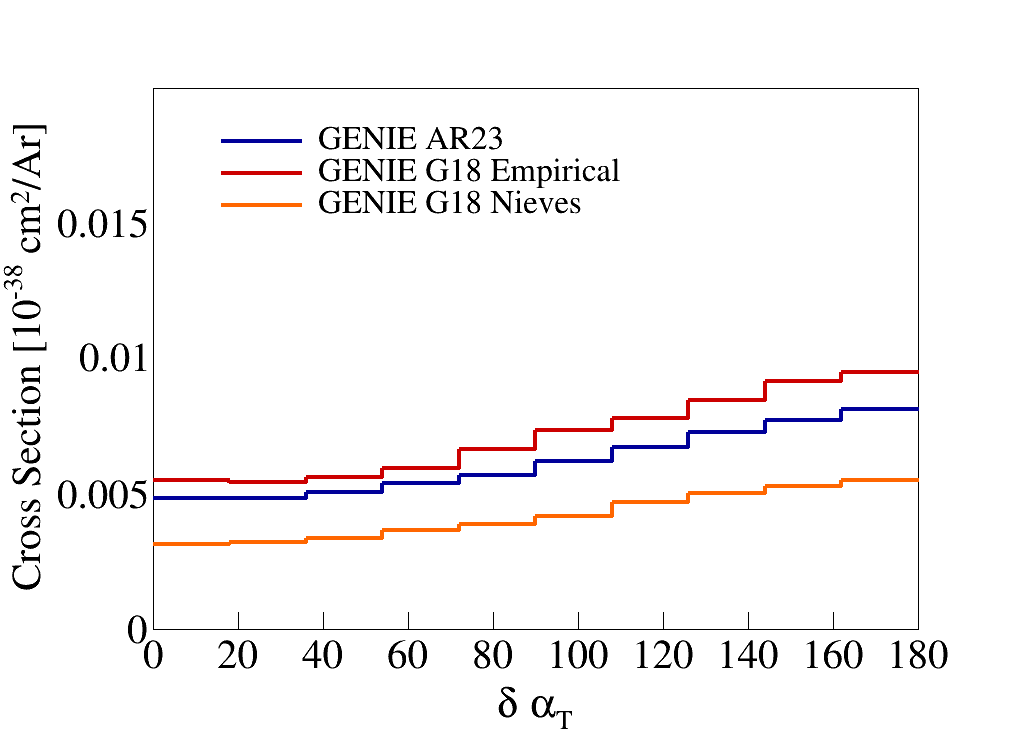
\includegraphics[width=3in]{Figs/Overlay/MEC/Overlay_TrueDeltaAlphaTPlot.png}} \\
    \subfloat{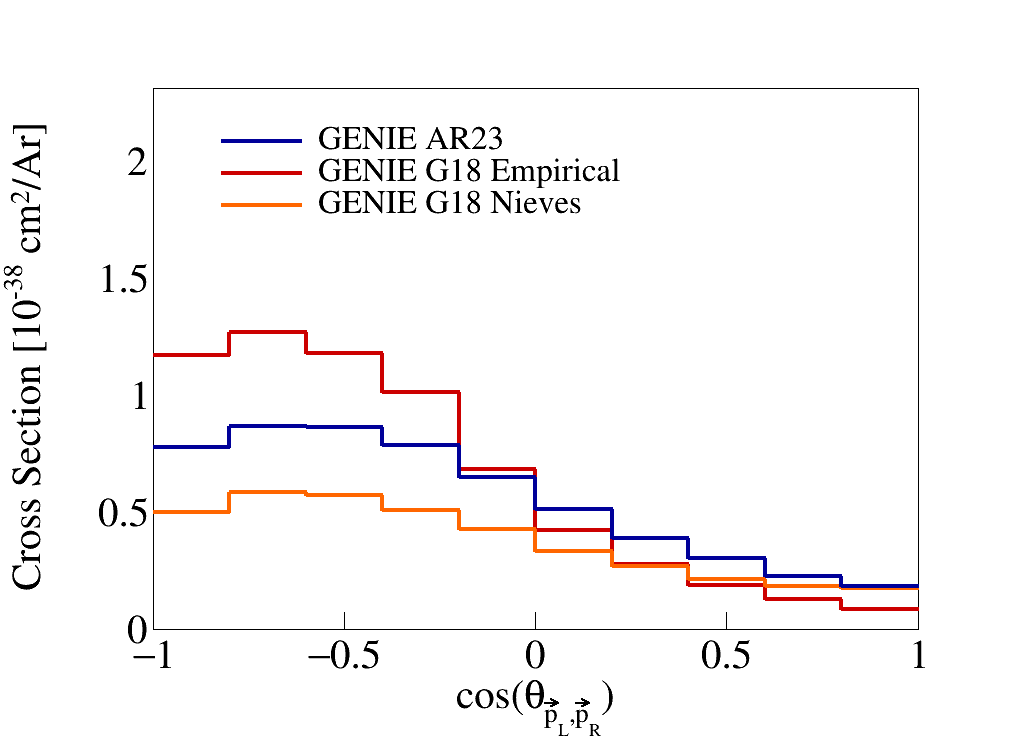
\includegraphics[width=3in]{Figs/Overlay/MEC/Overlay_TrueCosOpeningAngleProtonsPlot.png}}
    \subfloat{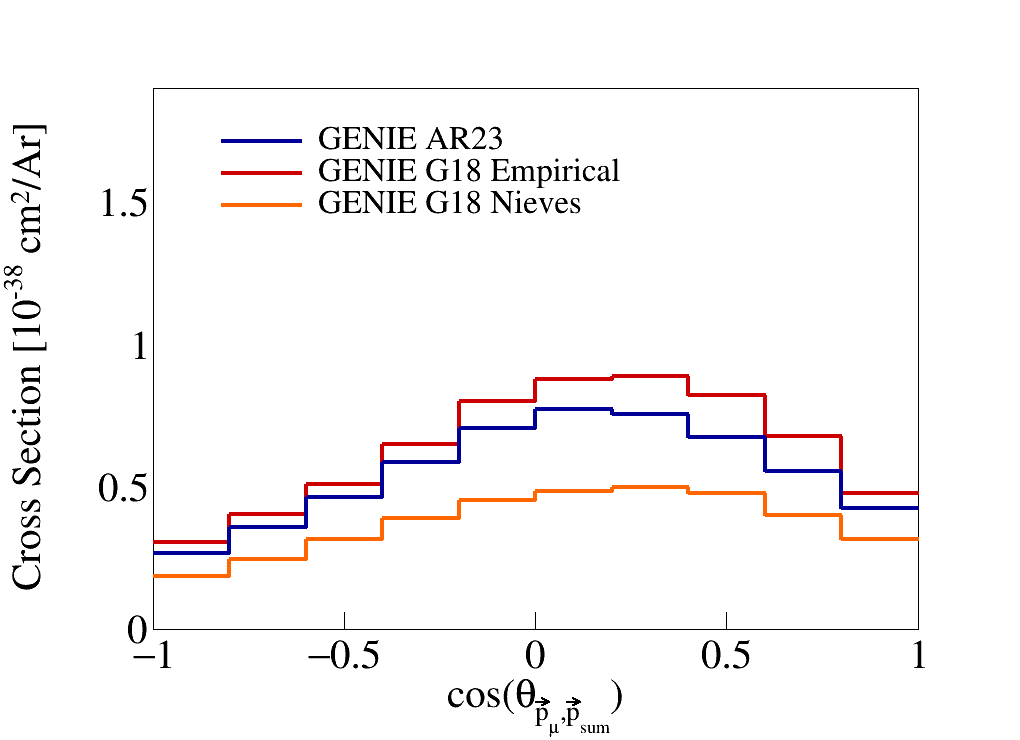
\includegraphics[width=3in]{Figs/Overlay/MEC/Overlay_TrueCosOpeningAngleMuonTotalProtonPlot.png}}
    \caption{Transverse kinematic variables for pure MEC events}
    \label{fig:transverse-k-mec}
\end{figure}

\begin{figure}
    \centering
    \subfloat{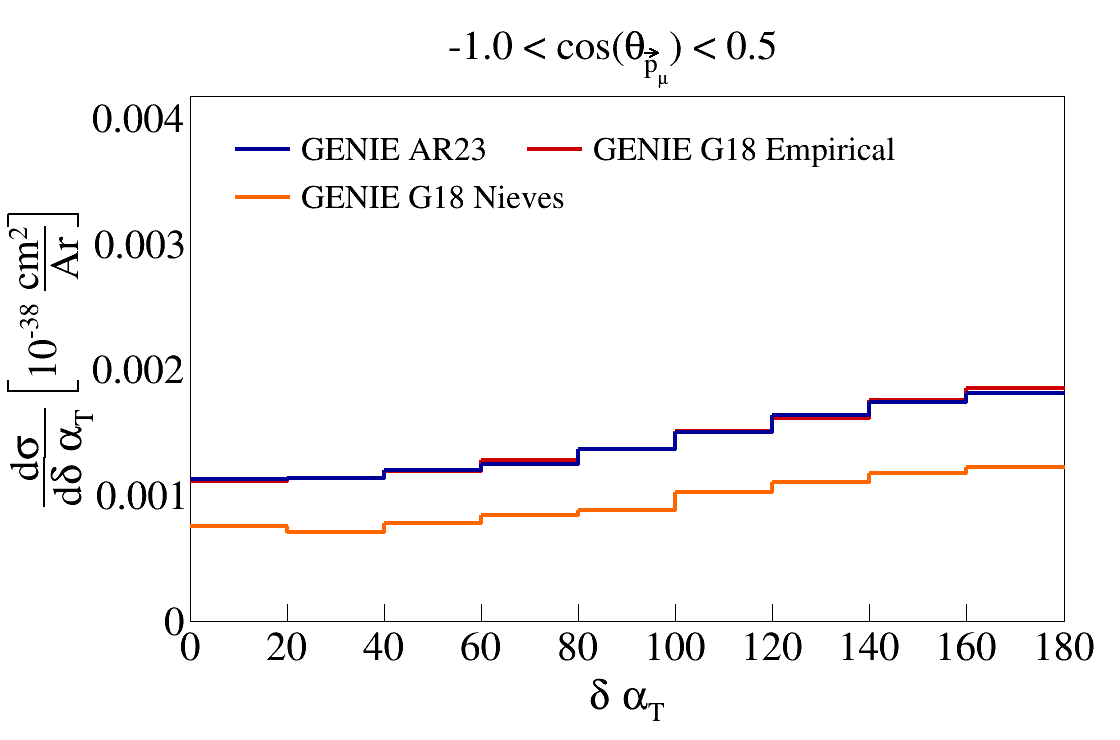
\includegraphics[width=3in]{Figs/Overlay/MEC/Serial/TrueSerialDeltaAlphaT_InMuonCosThetaPlot_0.png}}
    \subfloat{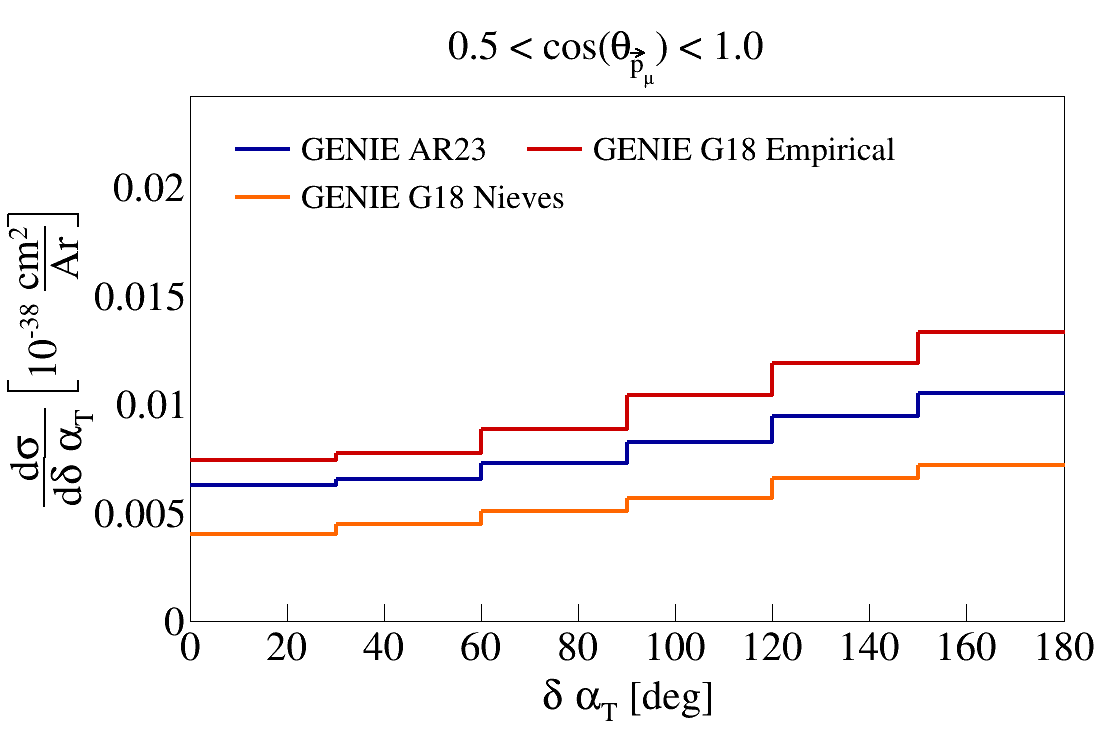
\includegraphics[width=3in]{Figs/Overlay/MEC/Serial/TrueSerialDeltaAlphaT_InMuonCosThetaPlot_1.png}} \\
    \subfloat{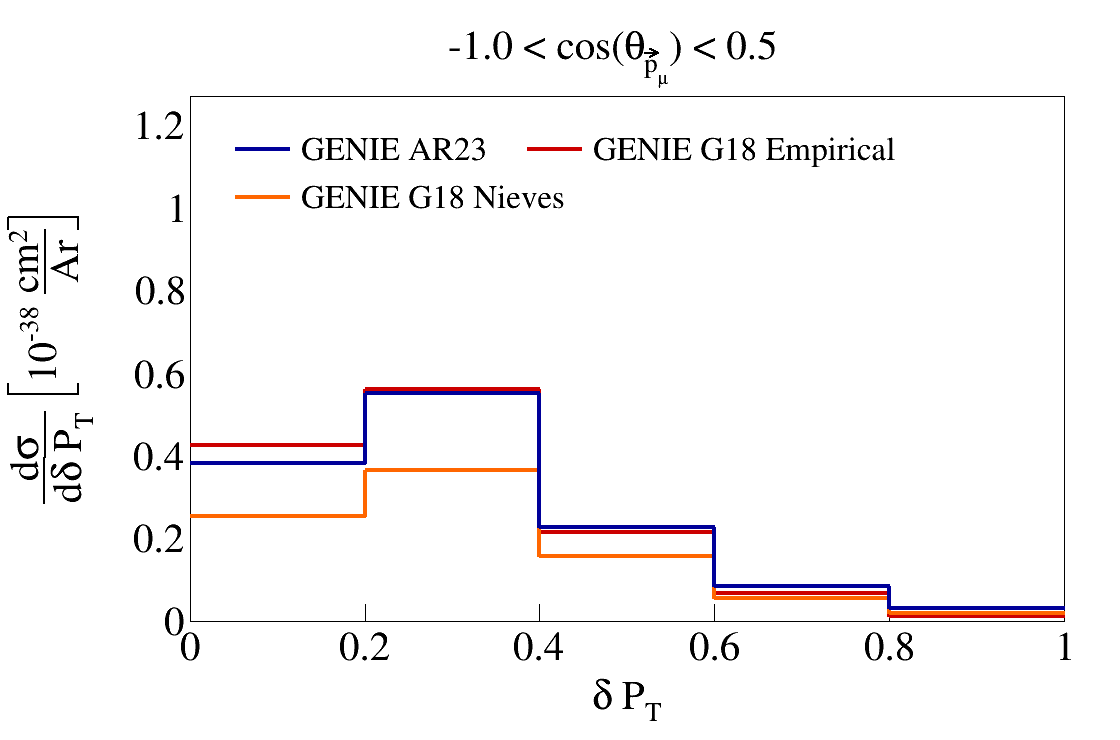
\includegraphics[width=3in]{Figs/Overlay/MEC/Serial/TrueSerialTransverseMomentum_InMuonCosThetaPlot_0.png}}
    \subfloat{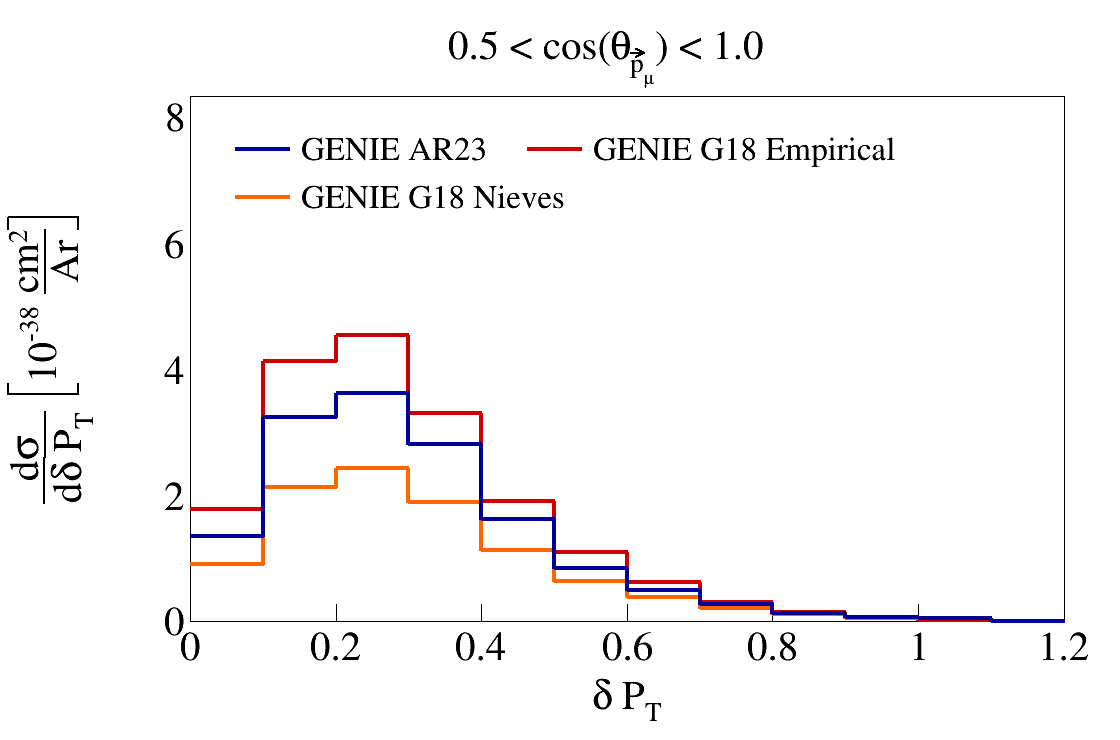
\includegraphics[width=3in]{Figs/Overlay/MEC/Serial/TrueSerialTransverseMomentum_InMuonCosThetaPlot_1.png}} \\
    \subfloat{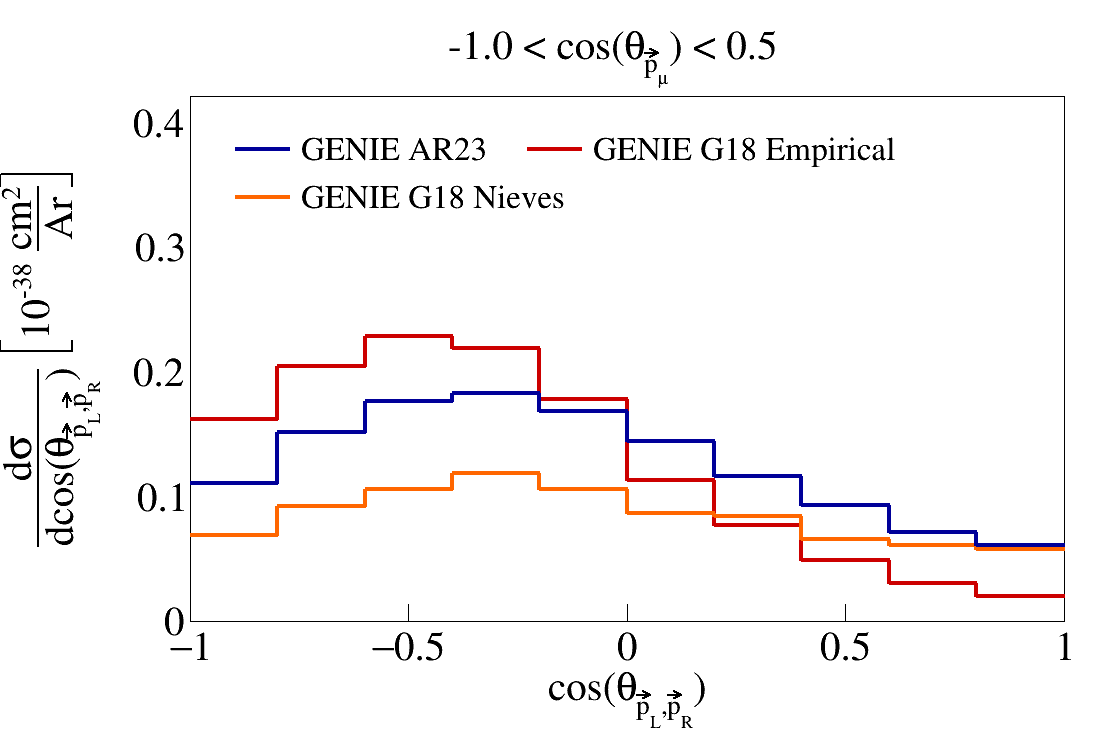
\includegraphics[width=3in]{Figs/Overlay/MEC/Serial/TrueSerialCosOpeningAngleProtons_InMuonCosThetaPlot_0.png}}
    \subfloat{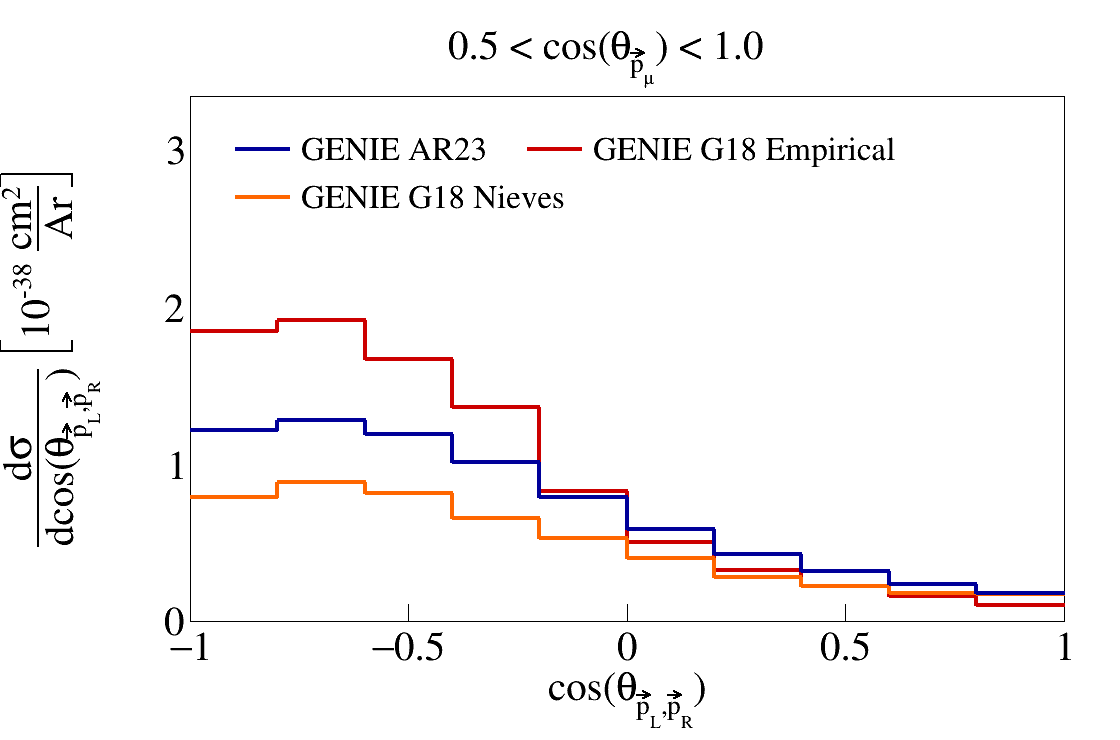
\includegraphics[width=3in]{Figs/Overlay/MEC/Serial/TrueSerialCosOpeningAngleProtons_InMuonCosThetaPlot_1.png}} \\
    \subfloat{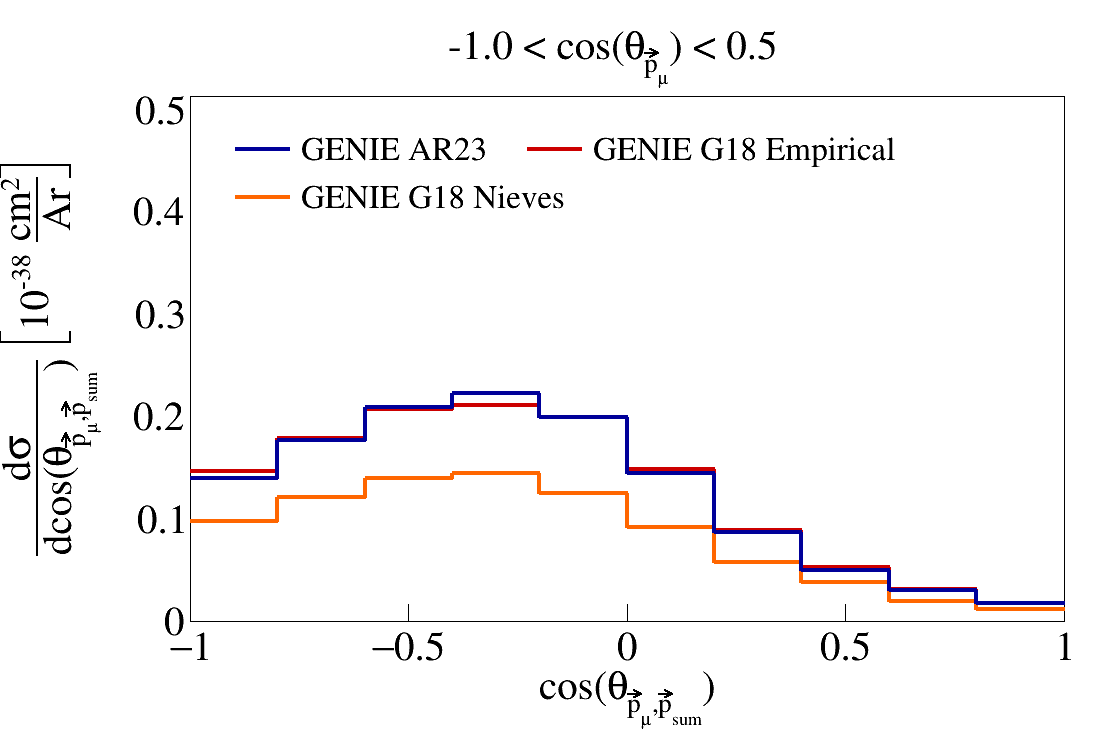
\includegraphics[width=3in]{Figs/Overlay/MEC/Serial/TrueSerialCosOpeningAngleMuonTotalProton_InMuonCosThetaPlot_0.png}}
    \subfloat{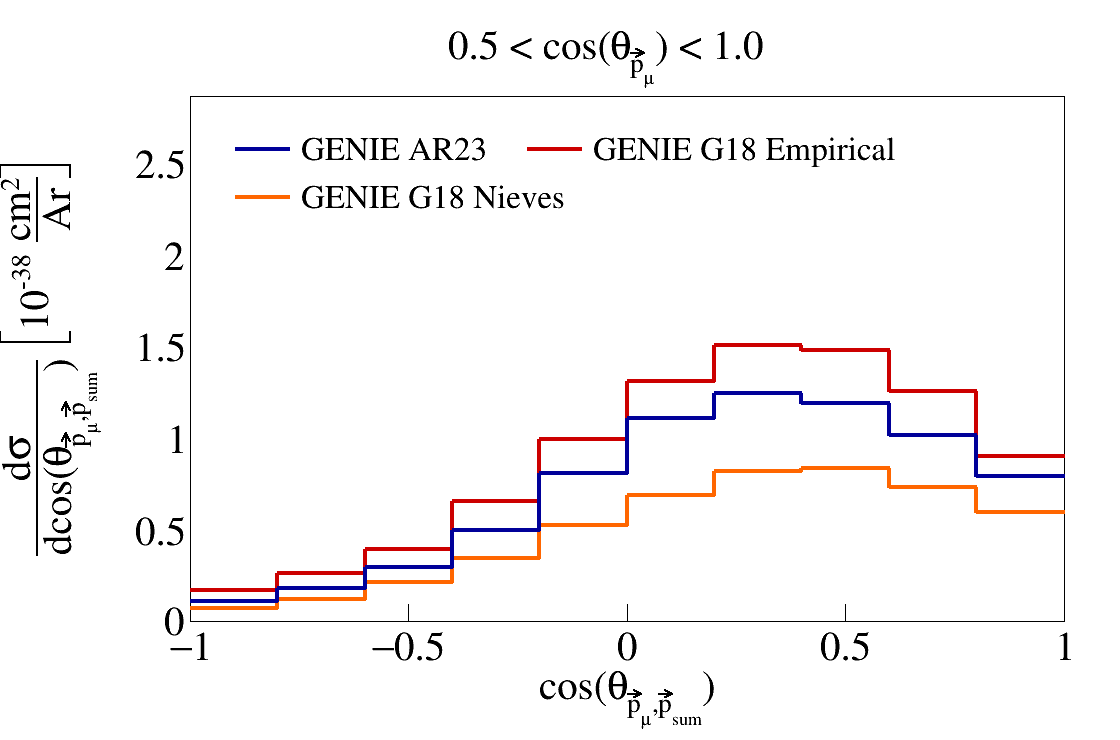
\includegraphics[width=3in]{Figs/Overlay/MEC/Serial/TrueSerialCosOpeningAngleMuonTotalProton_InMuonCosThetaPlot_1.png}} 
    \caption{Sliced double differential plots for pure MEC events}
    \label{fig:sliced-double-mec}
\end{figure}

\section{CAFAna analysis}

To perform analysis on experiment data, we will be using the CAFAna framework. 

\end{document}
